% Options for packages loaded elsewhere
\PassOptionsToPackage{unicode}{hyperref}
\PassOptionsToPackage{hyphens}{url}
\PassOptionsToPackage{dvipsnames,svgnames,x11names}{xcolor}
%
\documentclass[
  letterpaper,
  DIV=11,
  numbers=noendperiod]{scrreprt}
\usepackage{amsmath,amssymb}
\usepackage{lmodern}
\usepackage{iftex}
\ifPDFTeX
  \usepackage[T1]{fontenc}
  \usepackage[utf8]{inputenc}
  \usepackage{textcomp} % provide euro and other symbols
\else % if luatex or xetex
  \usepackage{unicode-math}
  \defaultfontfeatures{Scale=MatchLowercase}
  \defaultfontfeatures[\rmfamily]{Ligatures=TeX,Scale=1}
\fi
% Use upquote if available, for straight quotes in verbatim environments
\IfFileExists{upquote.sty}{\usepackage{upquote}}{}
\IfFileExists{microtype.sty}{% use microtype if available
  \usepackage[]{microtype}
  \UseMicrotypeSet[protrusion]{basicmath} % disable protrusion for tt fonts
}{}
\makeatletter
\@ifundefined{KOMAClassName}{% if non-KOMA class
  \IfFileExists{parskip.sty}{%
    \usepackage{parskip}
  }{% else
    \setlength{\parindent}{0pt}
    \setlength{\parskip}{6pt plus 2pt minus 1pt}}
}{% if KOMA class
  \KOMAoptions{parskip=half}}
\makeatother
\usepackage{xcolor}
\IfFileExists{xurl.sty}{\usepackage{xurl}}{} % add URL line breaks if available
\IfFileExists{bookmark.sty}{\usepackage{bookmark}}{\usepackage{hyperref}}
\hypersetup{
  pdftitle={My Document},
  pdfauthor={Bo Burla},
  colorlinks=true,
  linkcolor={blue},
  filecolor={Maroon},
  citecolor={Blue},
  urlcolor={Blue},
  pdfcreator={LaTeX via pandoc}}
\urlstyle{same} % disable monospaced font for URLs
\usepackage[normalem]{ulem}
% Avoid problems with \sout in headers with hyperref
\pdfstringdefDisableCommands{\renewcommand{\sout}{}}
\setlength{\emergencystretch}{3em} % prevent overfull lines
\setcounter{secnumdepth}{5}
% Make \paragraph and \subparagraph free-standing
\ifx\paragraph\undefined\else
  \let\oldparagraph\paragraph
  \renewcommand{\paragraph}[1]{\oldparagraph{#1}\mbox{}}
\fi
\ifx\subparagraph\undefined\else
  \let\oldsubparagraph\subparagraph
  \renewcommand{\subparagraph}[1]{\oldsubparagraph{#1}\mbox{}}
\fi

\usepackage{color}
\usepackage{fancyvrb}
\newcommand{\VerbBar}{|}
\newcommand{\VERB}{\Verb[commandchars=\\\{\}]}
\DefineVerbatimEnvironment{Highlighting}{Verbatim}{commandchars=\\\{\}}
% Add ',fontsize=\small' for more characters per line
\usepackage{framed}
\definecolor{shadecolor}{RGB}{241,243,245}
\newenvironment{Shaded}{\begin{snugshade}}{\end{snugshade}}
\newcommand{\AlertTok}[1]{\textcolor[rgb]{0.68,0.00,0.00}{#1}}
\newcommand{\AnnotationTok}[1]{\textcolor[rgb]{0.37,0.37,0.37}{#1}}
\newcommand{\AttributeTok}[1]{\textcolor[rgb]{0.40,0.45,0.13}{#1}}
\newcommand{\BaseNTok}[1]{\textcolor[rgb]{0.68,0.00,0.00}{#1}}
\newcommand{\BuiltInTok}[1]{\textcolor[rgb]{0.00,0.23,0.31}{#1}}
\newcommand{\CharTok}[1]{\textcolor[rgb]{0.13,0.47,0.30}{#1}}
\newcommand{\CommentTok}[1]{\textcolor[rgb]{0.37,0.37,0.37}{#1}}
\newcommand{\CommentVarTok}[1]{\textcolor[rgb]{0.37,0.37,0.37}{\textit{#1}}}
\newcommand{\ConstantTok}[1]{\textcolor[rgb]{0.56,0.35,0.01}{#1}}
\newcommand{\ControlFlowTok}[1]{\textcolor[rgb]{0.00,0.23,0.31}{#1}}
\newcommand{\DataTypeTok}[1]{\textcolor[rgb]{0.68,0.00,0.00}{#1}}
\newcommand{\DecValTok}[1]{\textcolor[rgb]{0.68,0.00,0.00}{#1}}
\newcommand{\DocumentationTok}[1]{\textcolor[rgb]{0.37,0.37,0.37}{\textit{#1}}}
\newcommand{\ErrorTok}[1]{\textcolor[rgb]{0.68,0.00,0.00}{#1}}
\newcommand{\ExtensionTok}[1]{\textcolor[rgb]{0.00,0.23,0.31}{#1}}
\newcommand{\FloatTok}[1]{\textcolor[rgb]{0.68,0.00,0.00}{#1}}
\newcommand{\FunctionTok}[1]{\textcolor[rgb]{0.28,0.35,0.67}{#1}}
\newcommand{\ImportTok}[1]{\textcolor[rgb]{0.00,0.46,0.62}{#1}}
\newcommand{\InformationTok}[1]{\textcolor[rgb]{0.37,0.37,0.37}{#1}}
\newcommand{\KeywordTok}[1]{\textcolor[rgb]{0.00,0.23,0.31}{#1}}
\newcommand{\NormalTok}[1]{\textcolor[rgb]{0.00,0.23,0.31}{#1}}
\newcommand{\OperatorTok}[1]{\textcolor[rgb]{0.37,0.37,0.37}{#1}}
\newcommand{\OtherTok}[1]{\textcolor[rgb]{0.00,0.23,0.31}{#1}}
\newcommand{\PreprocessorTok}[1]{\textcolor[rgb]{0.68,0.00,0.00}{#1}}
\newcommand{\RegionMarkerTok}[1]{\textcolor[rgb]{0.00,0.23,0.31}{#1}}
\newcommand{\SpecialCharTok}[1]{\textcolor[rgb]{0.37,0.37,0.37}{#1}}
\newcommand{\SpecialStringTok}[1]{\textcolor[rgb]{0.13,0.47,0.30}{#1}}
\newcommand{\StringTok}[1]{\textcolor[rgb]{0.13,0.47,0.30}{#1}}
\newcommand{\VariableTok}[1]{\textcolor[rgb]{0.07,0.07,0.07}{#1}}
\newcommand{\VerbatimStringTok}[1]{\textcolor[rgb]{0.13,0.47,0.30}{#1}}
\newcommand{\WarningTok}[1]{\textcolor[rgb]{0.37,0.37,0.37}{\textit{#1}}}

\providecommand{\tightlist}{%
  \setlength{\itemsep}{0pt}\setlength{\parskip}{0pt}}\usepackage{longtable,booktabs,array}
\usepackage{calc} % for calculating minipage widths
% Correct order of tables after \paragraph or \subparagraph
\usepackage{etoolbox}
\makeatletter
\patchcmd\longtable{\par}{\if@noskipsec\mbox{}\fi\par}{}{}
\makeatother
% Allow footnotes in longtable head/foot
\IfFileExists{footnotehyper.sty}{\usepackage{footnotehyper}}{\usepackage{footnote}}
\makesavenoteenv{longtable}
\usepackage{graphicx}
\makeatletter
\def\maxwidth{\ifdim\Gin@nat@width>\linewidth\linewidth\else\Gin@nat@width\fi}
\def\maxheight{\ifdim\Gin@nat@height>\textheight\textheight\else\Gin@nat@height\fi}
\makeatother
% Scale images if necessary, so that they will not overflow the page
% margins by default, and it is still possible to overwrite the defaults
% using explicit options in \includegraphics[width, height, ...]{}
\setkeys{Gin}{width=\maxwidth,height=\maxheight,keepaspectratio}
% Set default figure placement to htbp
\makeatletter
\def\fps@figure{htbp}
\makeatother
\newlength{\cslhangindent}
\setlength{\cslhangindent}{1.5em}
\newlength{\csllabelwidth}
\setlength{\csllabelwidth}{3em}
\newlength{\cslentryspacingunit} % times entry-spacing
\setlength{\cslentryspacingunit}{\parskip}
\newenvironment{CSLReferences}[2] % #1 hanging-ident, #2 entry spacing
 {% don't indent paragraphs
  \setlength{\parindent}{0pt}
  % turn on hanging indent if param 1 is 1
  \ifodd #1
  \let\oldpar\par
  \def\par{\hangindent=\cslhangindent\oldpar}
  \fi
  % set entry spacing
  \setlength{\parskip}{#2\cslentryspacingunit}
 }%
 {}
\usepackage{calc}
\newcommand{\CSLBlock}[1]{#1\hfill\break}
\newcommand{\CSLLeftMargin}[1]{\parbox[t]{\csllabelwidth}{#1}}
\newcommand{\CSLRightInline}[1]{\parbox[t]{\linewidth - \csllabelwidth}{#1}\break}
\newcommand{\CSLIndent}[1]{\hspace{\cslhangindent}#1}

\KOMAoption{captions}{tableheading}
\makeatletter
\makeatother
\makeatletter
\@ifpackageloaded{caption}{}{\usepackage{caption}}
\AtBeginDocument{%
\ifdefined\contentsname
  \renewcommand*\contentsname{Table of contents}
\else
  \newcommand\contentsname{Table of contents}
\fi
\ifdefined\listfigurename
  \renewcommand*\listfigurename{List of Figures}
\else
  \newcommand\listfigurename{List of Figures}
\fi
\ifdefined\listtablename
  \renewcommand*\listtablename{List of Tables}
\else
  \newcommand\listtablename{List of Tables}
\fi
\ifdefined\figurename
  \renewcommand*\figurename{Figure}
\else
  \newcommand\figurename{Figure}
\fi
\ifdefined\tablename
  \renewcommand*\tablename{Table}
\else
  \newcommand\tablename{Table}
\fi
}
\@ifpackageloaded{float}{}{\usepackage{float}}
\floatstyle{ruled}
\@ifundefined{c@chapter}{\newfloat{codelisting}{h}{lop}}{\newfloat{codelisting}{h}{lop}[chapter]}
\floatname{codelisting}{Listing}
\newcommand*\listoflistings{\listof{codelisting}{List of Listings}}
\makeatother
\makeatletter
\@ifpackageloaded{caption}{}{\usepackage{caption}}
\@ifpackageloaded{subcaption}{}{\usepackage{subcaption}}
\makeatother
\makeatletter
\@ifpackageloaded{tcolorbox}{}{\usepackage[many]{tcolorbox}}
\makeatother
\makeatletter
\@ifundefined{shadecolor}{\definecolor{shadecolor}{rgb}{.97, .97, .97}}
\makeatother
\makeatletter
\makeatother
\ifLuaTeX
  \usepackage{selnolig}  % disable illegal ligatures
\fi

\title{My Document}
\author{Bo Burla}
\date{5/13/2022}

\begin{document}
\maketitle

\ifdefined\Shaded\renewenvironment{Shaded}{\begin{tcolorbox}[interior hidden, boxrule=0pt, breakable, enhanced, sharp corners, frame hidden, borderline west={3pt}{0pt}{shadecolor}]}{\end{tcolorbox}}\fi

\renewcommand*\contentsname{Table of contents}
{
\hypersetup{linkcolor=}
\setcounter{tocdepth}{2}
\tableofcontents
}
\hypertarget{welcome}{%
\chapter*{Welcome}\label{welcome}}
\addcontentsline{toc}{chapter}{Welcome}

In this online book you will find the workshop notes of the RwithSLING
workshop sessions 2022 at the Singapore Lipidomics Incubator (SLING ) @
National University of Singapore.

These RwithSLING workshop sessions are aimed as quick-start in the
applied usage of R in data processing, management and analysis of
dataset handled in the lab. The focus of these sessions are on mass
spectrometry (MS)-based lipidomics and metabolomics datasets.

These notes were mainly prepared before and especially after each
workshop session, covering topics, challenges, pitfalls and solutions
discussed among all participants during the sessions.

Feedback and contributions are very welcome!

\hypertarget{introduction}{%
\chapter{Introduction}\label{introduction}}

\hypertarget{prerequisites}{%
\section{Prerequisites}\label{prerequisites}}

Following software need to be installed on your computer to work with
the examples shown in this online book:

\begin{itemize}
\item
  \texttt{R} Version 4.0 (or higher) \url{https://www.r-project.org/} or
  \url{https://cran.rstudio.com/}

  Check your R version by running following command in your console:

\begin{Shaded}
\begin{Highlighting}[]
\FunctionTok{R.Version}\NormalTok{()}\SpecialCharTok{$}\NormalTok{version.string}
\end{Highlighting}
\end{Shaded}

\begin{verbatim}
[1] "R version 4.2.0 (2022-04-22 ucrt)"
\end{verbatim}
\item
  \texttt{RStudio} Version 2022.02 or higher
  \url{https://www.rstudio.com/products/rstudio/download/\#download}

  Check your \texttt{RStudio} version by either looking clicking
  \emph{About RStudio} under the menu \emph{Help}, or by running
  following command in your console

\begin{Shaded}
\begin{Highlighting}[]
\CommentTok{\#rstudioapi::versionInfo()$version}
\end{Highlighting}
\end{Shaded}
\end{itemize}

Following software are only needed for specific chapters/examples:

\begin{itemize}
\tightlist
\item
  \texttt{Git} \url{https://git-scm.com/downloads}
\item
  For Windows: \texttt{Rtools}
  \textless https://cran.r-project.org/bin/windows/Rtools/
\end{itemize}

\hypertarget{frequently-used-r-packages}{%
\section{Frequently used R packages}\label{frequently-used-r-packages}}

See also @ref(Installing R packages)

Following R packages will be often used in the given examples and it is
thus recommended to install them before starting with this book

\begin{itemize}
\tightlist
\item
  \texttt{here}
\item
  \texttt{tidyverse}(installs
  \texttt{ggplot2,\ dplyr,\ tidyr,\ tibble,\ readr,\ forcats,\ stringr,\ purrr})
\item
  \texttt{readxl}
\item
  \texttt{remotes}
\end{itemize}

Run this in your R command line to install these packages:

\begin{Shaded}
\begin{Highlighting}[]
\CommentTok{\#pkg\_list \textless{}{-} c("here", "tidyverse", "readxl", "remotes")}
\CommentTok{\#install.packages(pkg\_list)}
\end{Highlighting}
\end{Shaded}

\hypertarget{read-ms-datasets-into-r}{%
\chapter{Read MS datasets into R}\label{read-ms-datasets-into-r}}

In this workshop we will try to use datasets types and formats that we
often encounter during our work. In this chapter we explore how to
import different types of data, with a focus on pre-processed MS
datasets. Processed MS datasets refers to data exported from MS raw data
processing software, such as Agilent MassHunter, Sciex Multiquant,
MRMkit and LDA. These files containing signal intensities such as peak
areas for LC-based methods and intensities for FIA/shutgun methods.

\hypertarget{read-csv-files}{%
\section{Read CSV files}\label{read-csv-files}}

\hypertarget{read-a-perfect-csv-file}{%
\subsection{Read a perfect CSV file}\label{read-a-perfect-csv-file}}

One of the easiest ways to import data into R is via an CSV
(comman-separated values) file.

\begin{itemize}
\tightlist
\item
  The first row should contains the column names, all subsequent rows
  data/values
\item
  A typical format for omics data consists of rows corresponding to
  samples, and columns to compounds (features).
\item
  White spaces in before or after any text fields can (often will) cause
  issues downstream, therefore I suggest to trim whitespaces by setting
  \texttt{trim\_ws\ =\ TRUE}
\end{itemize}

\begin{Shaded}
\begin{Highlighting}[]
\NormalTok{data\_file\_path }\OtherTok{\textless{}{-}} \FunctionTok{here}\NormalTok{(}\StringTok{"data/Testdata\_Lipidomics\_flat\_wide.csv"}\NormalTok{)}
\NormalTok{d\_wide }\OtherTok{\textless{}{-}}\NormalTok{ readr}\SpecialCharTok{::}\FunctionTok{read\_csv}\NormalTok{(data\_file\_path, }\AttributeTok{trim\_ws =} \ConstantTok{TRUE}\NormalTok{)}
\CommentTok{\#\textgreater{} Rows: 215 Columns: 432}
\CommentTok{\#\textgreater{} {-}{-} Column specification {-}{-}{-}{-}{-}{-}{-}{-}{-}{-}{-}{-}{-}{-}{-}{-}{-}{-}{-}{-}{-}{-}{-}{-}{-}{-}{-}{-}{-}{-}{-}{-}{-}{-}{-}{-}{-}{-}{-}{-}{-}{-}{-}{-}{-}{-}{-}{-}{-}{-}{-}{-}{-}{-}{-}{-}}
\CommentTok{\#\textgreater{} Delimiter: ","}
\CommentTok{\#\textgreater{} chr    (3): DataFileme, SampleType, VialPosition}
\CommentTok{\#\textgreater{} dbl  (426): CE 14:0, CE 15:0, CE 16:0, CE 16:1, CE 16:2, CE 17:0, CE 17:1, C...}
\CommentTok{\#\textgreater{} lgl    (2): Cer d18:2/24:0, LPC 16:0}
\CommentTok{\#\textgreater{} dttm   (1): AcqTimeStamp}
\CommentTok{\#\textgreater{} }
\CommentTok{\#\textgreater{} i Use \textasciigrave{}spec()\textasciigrave{} to retrieve the full column specification for this data.}
\CommentTok{\#\textgreater{} i Specify the column types or set \textasciigrave{}show\_col\_types = FALSE\textasciigrave{} to quiet this message.}
\end{Highlighting}
\end{Shaded}

Have a look at the summary returned by \texttt{read\_csv}. When using
minimal set of parameters as above, \texttt{read\_csv} will \emph{guess}
the type of data each column contains. You see that the columns
DataFileme, SampleType, VialPosition are of the type \texttt{char,}
which stands for \emph{text} (\uline{\emph{char}}\emph{acter}) fields,
AcqTimeStamp is of type \texttt{dttm}, indicating \emph{date-time}, and
all other columns are of the type \texttt{\textless{}dbl\textgreater{}}
indicating (\emph{double} precision floating point) numbers.

If you print tables in the console or in R notebook (.Rmd) you get a
summary of the table including the columnn types.

\begin{Shaded}
\begin{Highlighting}[]
\NormalTok{d\_wide}
\CommentTok{\#\textgreater{} \# A tibble: 215 x 432}
\CommentTok{\#\textgreater{}   DataFileme     AcqTimeStamp        SampleType VialPosition \textasciigrave{}CE 14:0\textasciigrave{} \textasciigrave{}CE 15:0\textasciigrave{}}
\CommentTok{\#\textgreater{}   \textless{}chr\textgreater{}          \textless{}dttm\textgreater{}              \textless{}chr\textgreater{}      \textless{}chr\textgreater{}            \textless{}dbl\textgreater{}     \textless{}dbl\textgreater{}}
\CommentTok{\#\textgreater{} 1 001\_EQC\_TQC p\textasciitilde{} 2018{-}04{-}12 18:28:00 Sample     Vial 2            1532       515}
\CommentTok{\#\textgreater{} 2 002\_EQC\_TQC p\textasciitilde{} 2018{-}04{-}12 18:39:00 Sample     Vial 2            1029       911}
\CommentTok{\#\textgreater{} 3 003\_EQC\_TQC p\textasciitilde{} 2018{-}04{-}12 18:51:00 Sample     Vial 2             685       649}
\CommentTok{\#\textgreater{} 4 004\_EQC\_TQC p\textasciitilde{} 2018{-}04{-}12 19:02:00 Sample     Vial 2            1283       576}
\CommentTok{\#\textgreater{} \# ... with 211 more rows, and 426 more variables: \textasciigrave{}CE 16:0\textasciigrave{} \textless{}dbl\textgreater{},}
\CommentTok{\#\textgreater{} \#   \textasciigrave{}CE 16:1\textasciigrave{} \textless{}dbl\textgreater{}, \textasciigrave{}CE 16:2\textasciigrave{} \textless{}dbl\textgreater{}, \textasciigrave{}CE 17:0\textasciigrave{} \textless{}dbl\textgreater{}, \textasciigrave{}CE 17:1\textasciigrave{} \textless{}dbl\textgreater{},}
\CommentTok{\#\textgreater{} \#   \textasciigrave{}CE 18:0\textasciigrave{} \textless{}dbl\textgreater{}, \textasciigrave{}CE 18:1\textasciigrave{} \textless{}dbl\textgreater{}, \textasciigrave{}CE 18:1 d7 (ISTD)\textasciigrave{} \textless{}dbl\textgreater{},}
\CommentTok{\#\textgreater{} \#   \textasciigrave{}CE 18:2\textasciigrave{} \textless{}dbl\textgreater{}, \textasciigrave{}CE 18:3\textasciigrave{} \textless{}dbl\textgreater{}, \textasciigrave{}CE 20:1\textasciigrave{} \textless{}dbl\textgreater{}, \textasciigrave{}CE 20:2\textasciigrave{} \textless{}dbl\textgreater{},}
\CommentTok{\#\textgreater{} \#   \textasciigrave{}CE 20:3\textasciigrave{} \textless{}dbl\textgreater{}, \textasciigrave{}CE 20:4\textasciigrave{} \textless{}dbl\textgreater{}, \textasciigrave{}CE 20:5\textasciigrave{} \textless{}dbl\textgreater{}, \textasciigrave{}CE 22:0\textasciigrave{} \textless{}dbl\textgreater{},}
\CommentTok{\#\textgreater{} \#   \textasciigrave{}CE 22:1\textasciigrave{} \textless{}dbl\textgreater{}, \textasciigrave{}CE 22:4\textasciigrave{} \textless{}dbl\textgreater{}, \textasciigrave{}CE 22:5\textasciigrave{} \textless{}dbl\textgreater{}, \textasciigrave{}CE 22:6\textasciigrave{} \textless{}dbl\textgreater{},}
\CommentTok{\#\textgreater{} \#   \textasciigrave{}CE 24:4\textasciigrave{} \textless{}dbl\textgreater{}, \textasciigrave{}Cer d18:0/16:0\textasciigrave{} \textless{}dbl\textgreater{}, \textasciigrave{}Cer d18:0/18:0\textasciigrave{} \textless{}dbl\textgreater{}, ...}
\end{Highlighting}
\end{Shaded}

\hypertarget{read-csvs-with-missing-values}{%
\subsection{Read CSVs with missing
values}\label{read-csvs-with-missing-values}}

Data files can easily contain missing values. For example, if no peak
was detected no value returned, with the CSV file containing an empty
field. \texttt{read\_csv} assigns empty/missing values during the import
to the specific value \texttt{NA} (\emph{Not Available}). This will not
affect to data type of the columns.

However, it might be that your data file contains specific text for
missing values, for instance ``\emph{ND''},''\emph{LOD''} or lowercase
\emph{``na''}. In tables from clinical chemistry or other clinical
parameters, there are frequently exts such as \emph{``clotted''},
\emph{``hemolytic''}, \emph{``no received''} indicating when/why a value
was not reported. What happens when we import such a file?

\begin{Shaded}
\begin{Highlighting}[]
\NormalTok{data\_file\_path }\OtherTok{\textless{}{-}} \FunctionTok{here}\NormalTok{(}\StringTok{"data/Testdata\_Lipidomics\_flat\_wide\_with\_differentNA.csv"}\NormalTok{)}
\NormalTok{d\_wide }\OtherTok{\textless{}{-}}\NormalTok{ readr}\SpecialCharTok{::}\FunctionTok{read\_csv}\NormalTok{(data\_file\_path, }\AttributeTok{trim\_ws =} \ConstantTok{TRUE}\NormalTok{)}
\CommentTok{\#\textgreater{} Rows: 215 Columns: 432}
\CommentTok{\#\textgreater{} {-}{-} Column specification {-}{-}{-}{-}{-}{-}{-}{-}{-}{-}{-}{-}{-}{-}{-}{-}{-}{-}{-}{-}{-}{-}{-}{-}{-}{-}{-}{-}{-}{-}{-}{-}{-}{-}{-}{-}{-}{-}{-}{-}{-}{-}{-}{-}{-}{-}{-}{-}{-}{-}{-}{-}{-}{-}{-}{-}}
\CommentTok{\#\textgreater{} Delimiter: ","}
\CommentTok{\#\textgreater{} chr  (109): DataFileNDme, SampleType, VialPosition, CE 15:0, CE 16:0, CE 17:...}
\CommentTok{\#\textgreater{} dbl  (320): CE 14:0, CE 16:1, CE 17:1, CE 18:0, CE 18:1, CE 18:1 d7 (ISTD), ...}
\CommentTok{\#\textgreater{} lgl    (2): CE 16:2, LPC 16:0}
\CommentTok{\#\textgreater{} dttm   (1): AcqTimeStamp}
\CommentTok{\#\textgreater{} }
\CommentTok{\#\textgreater{} i Use \textasciigrave{}spec()\textasciigrave{} to retrieve the full column specification for this data.}
\CommentTok{\#\textgreater{} i Specify the column types or set \textasciigrave{}show\_col\_types = FALSE\textasciigrave{} to quiet this message.}
\end{Highlighting}
\end{Shaded}

\texttt{read\_csv} was mislead by the presence of unknown text values
and guessed the data types wrongly as
\texttt{\textless{}char\textgreater{}} for some columns as text instead
of numbers. We also have two columns of the type
\texttt{\textless{}lgl\textgreater{}}, which stand for logical
(\texttt{TRUE}/\texttt{FALSE}), what happend here? All peak areas of
e.g.~CE 16:2 were missing and \texttt{read\_csv} has no way to guess
what is the intended data type, in which case it chooses
\texttt{\textless{}lgl\textgreater{}}as default.

We will not be able to perform any calculations for columns that are
text or logical. We therefore need to explicitly tell R what values to
interpret as missing values (\texttt{NA}). We can do this by providing a
list of texts that should be interpreted as \texttt{NA} using the the
\texttt{na} parameter. In the example below we consider ND and LOD as
missing values and they will be assing the standard \texttt{NA}. Note
that you can either have values or missing values, there is no way to
have different types of missing values in the standard R data table
formats.

\begin{Shaded}
\begin{Highlighting}[]
\NormalTok{data\_file\_path }\OtherTok{\textless{}{-}} \FunctionTok{here}\NormalTok{(}\StringTok{"data/Testdata\_Lipidomics\_flat\_wide\_with\_differentNA.csv"}\NormalTok{)}
\NormalTok{d\_wide }\OtherTok{\textless{}{-}}\NormalTok{ readr}\SpecialCharTok{::}\FunctionTok{read\_csv}\NormalTok{(data\_file\_path, }\AttributeTok{trim\_ws =} \ConstantTok{TRUE}\NormalTok{, }\AttributeTok{na =} \FunctionTok{c}\NormalTok{(}\StringTok{"ND"}\NormalTok{, }\StringTok{"LOD"}\NormalTok{))}
\CommentTok{\#\textgreater{} Warning: One or more parsing issues, see \textasciigrave{}problems()\textasciigrave{} for details}
\CommentTok{\#\textgreater{} Rows: 215 Columns: 432}
\CommentTok{\#\textgreater{} {-}{-} Column specification {-}{-}{-}{-}{-}{-}{-}{-}{-}{-}{-}{-}{-}{-}{-}{-}{-}{-}{-}{-}{-}{-}{-}{-}{-}{-}{-}{-}{-}{-}{-}{-}{-}{-}{-}{-}{-}{-}{-}{-}{-}{-}{-}{-}{-}{-}{-}{-}{-}{-}{-}{-}{-}{-}{-}{-}}
\CommentTok{\#\textgreater{} Delimiter: ","}
\CommentTok{\#\textgreater{} chr    (3): DataFileNDme, SampleType, VialPosition}
\CommentTok{\#\textgreater{} dbl  (425): CE 14:0, CE 15:0, CE 16:0, CE 16:1, CE 17:0, CE 17:1, CE 18:0, C...}
\CommentTok{\#\textgreater{} lgl    (3): CE 16:2, Cer d18:2/24:0, LPC 16:0}
\CommentTok{\#\textgreater{} dttm   (1): AcqTimeStamp}
\CommentTok{\#\textgreater{} }
\CommentTok{\#\textgreater{} i Use \textasciigrave{}spec()\textasciigrave{} to retrieve the full column specification for this data.}
\CommentTok{\#\textgreater{} i Specify the column types or set \textasciigrave{}show\_col\_types = FALSE\textasciigrave{} to quiet this message.}
\FunctionTok{print}\NormalTok{(d\_wide)}
\CommentTok{\#\textgreater{} \# A tibble: 215 x 432}
\CommentTok{\#\textgreater{}   DataFileNDme   AcqTimeStamp        SampleType VialPosition \textasciigrave{}CE 14:0\textasciigrave{} \textasciigrave{}CE 15:0\textasciigrave{}}
\CommentTok{\#\textgreater{}   \textless{}chr\textgreater{}          \textless{}dttm\textgreater{}              \textless{}chr\textgreater{}      \textless{}chr\textgreater{}            \textless{}dbl\textgreater{}     \textless{}dbl\textgreater{}}
\CommentTok{\#\textgreater{} 1 001\_EQC\_TQC p\textasciitilde{} 2018{-}04{-}12 18:28:00 Sample     Vial 2            1532       515}
\CommentTok{\#\textgreater{} 2 002\_EQC\_TQC p\textasciitilde{} 2018{-}04{-}12 18:39:00 Sample     Vial 2            1029        NA}
\CommentTok{\#\textgreater{} 3 003\_EQC\_TQC p\textasciitilde{} 2018{-}04{-}12 18:51:00 Sample     Vial 2             685       649}
\CommentTok{\#\textgreater{} 4 004\_EQC\_TQC p\textasciitilde{} 2018{-}04{-}12 19:02:00 Sample     Vial 2            1283       576}
\CommentTok{\#\textgreater{} \# ... with 211 more rows, and 426 more variables: \textasciigrave{}CE 16:0\textasciigrave{} \textless{}dbl\textgreater{},}
\CommentTok{\#\textgreater{} \#   \textasciigrave{}CE 16:1\textasciigrave{} \textless{}dbl\textgreater{}, \textasciigrave{}CE 16:2\textasciigrave{} \textless{}lgl\textgreater{}, \textasciigrave{}CE 17:0\textasciigrave{} \textless{}dbl\textgreater{}, \textasciigrave{}CE 17:1\textasciigrave{} \textless{}dbl\textgreater{},}
\CommentTok{\#\textgreater{} \#   \textasciigrave{}CE 18:0\textasciigrave{} \textless{}dbl\textgreater{}, \textasciigrave{}CE 18:1\textasciigrave{} \textless{}dbl\textgreater{}, \textasciigrave{}CE 18:1 d7 (ISTD)\textasciigrave{} \textless{}dbl\textgreater{},}
\CommentTok{\#\textgreater{} \#   \textasciigrave{}CE 18:2\textasciigrave{} \textless{}dbl\textgreater{}, \textasciigrave{}CE 18:3\textasciigrave{} \textless{}dbl\textgreater{}, \textasciigrave{}CE 20:1\textasciigrave{} \textless{}dbl\textgreater{}, \textasciigrave{}CE 20:2\textasciigrave{} \textless{}dbl\textgreater{},}
\CommentTok{\#\textgreater{} \#   \textasciigrave{}CE 20:3\textasciigrave{} \textless{}dbl\textgreater{}, \textasciigrave{}CE 20:4\textasciigrave{} \textless{}dbl\textgreater{}, \textasciigrave{}CE 20:5\textasciigrave{} \textless{}dbl\textgreater{}, \textasciigrave{}CE 22:0\textasciigrave{} \textless{}dbl\textgreater{},}
\CommentTok{\#\textgreater{} \#   \textasciigrave{}CE 22:1\textasciigrave{} \textless{}dbl\textgreater{}, \textasciigrave{}CE 22:4\textasciigrave{} \textless{}dbl\textgreater{}, \textasciigrave{}CE 22:5\textasciigrave{} \textless{}dbl\textgreater{}, \textasciigrave{}CE 22:6\textasciigrave{} \textless{}dbl\textgreater{},}
\CommentTok{\#\textgreater{} \#   \textasciigrave{}CE 24:4\textasciigrave{} \textless{}dbl\textgreater{}, \textasciigrave{}Cer d18:0/16:0\textasciigrave{} \textless{}dbl\textgreater{}, \textasciigrave{}Cer d18:0/18:0\textasciigrave{} \textless{}dbl\textgreater{}, ...}
\end{Highlighting}
\end{Shaded}

\hypertarget{importing-an-excel-table}{%
\section{Importing an Excel table}\label{importing-an-excel-table}}

A flat Excel table with features (e.g.~lipids, compounds) in columns,
and samples as rows can also be directly imported into R. Note that you
will need to define which sheet to import (e.g.~below \texttt{Sheet1}).
Also here, I suggest to trim white spaces by setting the
\texttt{trim\_ws} parameter to \texttt{TRUE}. The same aspects
concerning missing values as decribed in the previous section applies
when it comes to missing values. Also the \texttt{read\_xls} function
offers the \texttt{na} parameter.

\begin{Shaded}
\begin{Highlighting}[]
\NormalTok{data\_file\_path }\OtherTok{\textless{}{-}} \FunctionTok{here}\NormalTok{(}\StringTok{"data/Testdata\_Lipidomics\_flat\_wide.xlsx"}\NormalTok{)}
\NormalTok{d\_wide }\OtherTok{\textless{}{-}}\NormalTok{ readxl}\SpecialCharTok{::}\FunctionTok{read\_xlsx}\NormalTok{(data\_file\_path,}\AttributeTok{sheet =} \StringTok{"Sheet1"}\NormalTok{,}\AttributeTok{trim\_ws =} \ConstantTok{TRUE}\NormalTok{, }\AttributeTok{na =} \FunctionTok{c}\NormalTok{(}\StringTok{"ND"}\NormalTok{))}
\FunctionTok{print}\NormalTok{(d\_wide)}
\CommentTok{\#\textgreater{} \# A tibble: 215 x 432}
\CommentTok{\#\textgreater{}   DataFileName          AcqTimeStamp SampleType VialPosition \textasciigrave{}CE 14:0\textasciigrave{} \textasciigrave{}CE 15:0\textasciigrave{}}
\CommentTok{\#\textgreater{}   \textless{}chr\textgreater{}                 \textless{}chr\textgreater{}        \textless{}chr\textgreater{}      \textless{}chr\textgreater{}            \textless{}dbl\textgreater{}     \textless{}dbl\textgreater{}}
\CommentTok{\#\textgreater{} 1 001\_EQC\_TQC prerun 0\textasciitilde{} 2018{-}04{-}12T\textasciitilde{} Sample     Vial 2            1532       515}
\CommentTok{\#\textgreater{} 2 002\_EQC\_TQC prerun 0\textasciitilde{} 2018{-}04{-}12T\textasciitilde{} Sample     Vial 2            1029       911}
\CommentTok{\#\textgreater{} 3 003\_EQC\_TQC prerun 0\textasciitilde{} 2018{-}04{-}12T\textasciitilde{} Sample     Vial 2             685       649}
\CommentTok{\#\textgreater{} 4 004\_EQC\_TQC prerun 0\textasciitilde{} 2018{-}04{-}12T\textasciitilde{} Sample     Vial 2            1283       576}
\CommentTok{\#\textgreater{} \# ... with 211 more rows, and 426 more variables: \textasciigrave{}CE 16:0\textasciigrave{} \textless{}dbl\textgreater{},}
\CommentTok{\#\textgreater{} \#   \textasciigrave{}CE 16:1\textasciigrave{} \textless{}dbl\textgreater{}, \textasciigrave{}CE 16:2\textasciigrave{} \textless{}dbl\textgreater{}, \textasciigrave{}CE 17:0\textasciigrave{} \textless{}chr\textgreater{}, \textasciigrave{}CE 17:1\textasciigrave{} \textless{}dbl\textgreater{},}
\CommentTok{\#\textgreater{} \#   \textasciigrave{}CE 18:0\textasciigrave{} \textless{}dbl\textgreater{}, \textasciigrave{}CE 18:1\textasciigrave{} \textless{}dbl\textgreater{}, \textasciigrave{}CE 18:1 d7 (ISTD)\textasciigrave{} \textless{}dbl\textgreater{},}
\CommentTok{\#\textgreater{} \#   \textasciigrave{}CE 18:2\textasciigrave{} \textless{}dbl\textgreater{}, \textasciigrave{}CE 18:3\textasciigrave{} \textless{}dbl\textgreater{}, \textasciigrave{}CE 20:1\textasciigrave{} \textless{}chr\textgreater{}, \textasciigrave{}CE 20:2\textasciigrave{} \textless{}chr\textgreater{},}
\CommentTok{\#\textgreater{} \#   \textasciigrave{}CE 20:3\textasciigrave{} \textless{}dbl\textgreater{}, \textasciigrave{}CE 20:4\textasciigrave{} \textless{}dbl\textgreater{}, \textasciigrave{}CE 20:5\textasciigrave{} \textless{}dbl\textgreater{}, \textasciigrave{}CE 22:0\textasciigrave{} \textless{}dbl\textgreater{},}
\CommentTok{\#\textgreater{} \#   \textasciigrave{}CE 22:1\textasciigrave{} \textless{}dbl\textgreater{}, \textasciigrave{}CE 22:4\textasciigrave{} \textless{}chr\textgreater{}, \textasciigrave{}CE 22:5\textasciigrave{} \textless{}chr\textgreater{}, \textasciigrave{}CE 22:6\textasciigrave{} \textless{}dbl\textgreater{},}
\CommentTok{\#\textgreater{} \#   \textasciigrave{}CE 24:4\textasciigrave{} \textless{}chr\textgreater{}, \textasciigrave{}Cer d18:0/16:0\textasciigrave{} \textless{}dbl\textgreater{}, \textasciigrave{}Cer d18:0/18:0\textasciigrave{} \textless{}dbl\textgreater{}, ...}
\end{Highlighting}
\end{Shaded}

\hypertarget{import-peak-areas-from-agilent-masshunter-csv-file}{%
\section{Import peak areas from Agilent MassHunter CSV
file}\label{import-peak-areas-from-agilent-masshunter-csv-file}}

\begin{Shaded}
\begin{Highlighting}[]
\NormalTok{data\_file\_path }\OtherTok{\textless{}{-}} \FunctionTok{here}\NormalTok{(}\StringTok{"data/Testdata\_Lipidomics\_MHQuant\_Detailed.csv"}\NormalTok{)}
\NormalTok{d\_wide }\OtherTok{\textless{}{-}}\NormalTok{ SLINGtools}\SpecialCharTok{::}\FunctionTok{read\_peakareas\_MassHunterCSV}\NormalTok{(data\_file\_path)}
\CommentTok{\#\textgreater{} Reading \textquotesingle{}Testdata\_Lipidomics\_MHQuant\_Detailed.csv\textquotesingle{} ... }
\CommentTok{\#\textgreater{} Imported  215 samples with 428 transitions}
\FunctionTok{print}\NormalTok{(d\_wide)}
\CommentTok{\#\textgreater{} \# A tibble: 215 x 432}
\CommentTok{\#\textgreater{}   DataFileName   AcqTimeStamp        SampleType VialPosition \textasciigrave{}CE 14:0\textasciigrave{} \textasciigrave{}CE 15:0\textasciigrave{}}
\CommentTok{\#\textgreater{}   \textless{}chr\textgreater{}          \textless{}dttm\textgreater{}              \textless{}chr\textgreater{}      \textless{}chr\textgreater{}            \textless{}dbl\textgreater{}     \textless{}dbl\textgreater{}}
\CommentTok{\#\textgreater{} 1 001\_EQC\_TQC p\textasciitilde{} 2018{-}04{-}12 18:28:00 Sample     Vial 2            1532       515}
\CommentTok{\#\textgreater{} 2 002\_EQC\_TQC p\textasciitilde{} 2018{-}04{-}12 18:39:00 Sample     Vial 2            1029       911}
\CommentTok{\#\textgreater{} 3 003\_EQC\_TQC p\textasciitilde{} 2018{-}04{-}12 18:51:00 Sample     Vial 2             685       649}
\CommentTok{\#\textgreater{} 4 004\_EQC\_TQC p\textasciitilde{} 2018{-}04{-}12 19:02:00 Sample     Vial 2            1283       576}
\CommentTok{\#\textgreater{} \# ... with 211 more rows, and 426 more variables: \textasciigrave{}CE 16:0\textasciigrave{} \textless{}dbl\textgreater{},}
\CommentTok{\#\textgreater{} \#   \textasciigrave{}CE 16:1\textasciigrave{} \textless{}dbl\textgreater{}, \textasciigrave{}CE 16:2\textasciigrave{} \textless{}dbl\textgreater{}, \textasciigrave{}CE 17:0\textasciigrave{} \textless{}dbl\textgreater{}, \textasciigrave{}CE 17:1\textasciigrave{} \textless{}dbl\textgreater{},}
\CommentTok{\#\textgreater{} \#   \textasciigrave{}CE 18:0\textasciigrave{} \textless{}dbl\textgreater{}, \textasciigrave{}CE 18:1\textasciigrave{} \textless{}dbl\textgreater{}, \textasciigrave{}CE 18:1 d7 (ISTD)\textasciigrave{} \textless{}dbl\textgreater{},}
\CommentTok{\#\textgreater{} \#   \textasciigrave{}CE 18:2\textasciigrave{} \textless{}dbl\textgreater{}, \textasciigrave{}CE 18:3\textasciigrave{} \textless{}dbl\textgreater{}, \textasciigrave{}CE 20:1\textasciigrave{} \textless{}dbl\textgreater{}, \textasciigrave{}CE 20:2\textasciigrave{} \textless{}dbl\textgreater{},}
\CommentTok{\#\textgreater{} \#   \textasciigrave{}CE 20:3\textasciigrave{} \textless{}dbl\textgreater{}, \textasciigrave{}CE 20:4\textasciigrave{} \textless{}dbl\textgreater{}, \textasciigrave{}CE 20:5\textasciigrave{} \textless{}dbl\textgreater{}, \textasciigrave{}CE 22:0\textasciigrave{} \textless{}dbl\textgreater{},}
\CommentTok{\#\textgreater{} \#   \textasciigrave{}CE 22:1\textasciigrave{} \textless{}dbl\textgreater{}, \textasciigrave{}CE 22:4\textasciigrave{} \textless{}dbl\textgreater{}, \textasciigrave{}CE 22:5\textasciigrave{} \textless{}dbl\textgreater{}, \textasciigrave{}CE 22:6\textasciigrave{} \textless{}dbl\textgreater{},}
\CommentTok{\#\textgreater{} \#   \textasciigrave{}CE 24:4\textasciigrave{} \textless{}dbl\textgreater{}, \textasciigrave{}Cer d18:0/16:0\textasciigrave{} \textless{}dbl\textgreater{}, \textasciigrave{}Cer d18:0/18:0\textasciigrave{} \textless{}dbl\textgreater{}, ...}
\end{Highlighting}
\end{Shaded}

\hypertarget{import-all-data-from-an-agilent-masshunter-csv-file}{%
\section{Import all data from an Agilent MassHunter CSV
file}\label{import-all-data-from-an-agilent-masshunter-csv-file}}

\begin{Shaded}
\begin{Highlighting}[]
\NormalTok{data\_file\_path }\OtherTok{\textless{}{-}} \FunctionTok{here}\NormalTok{(}\StringTok{"data/Testdata\_Lipidomics\_MHQuant\_Detailed.csv"}\NormalTok{)}
\NormalTok{d\_all\_long }\OtherTok{\textless{}{-}}\NormalTok{ SLINGtools}\SpecialCharTok{::}\FunctionTok{read\_MassHunterCSV}\NormalTok{(data\_file\_path)}
\CommentTok{\#\textgreater{} Reading \textquotesingle{}Testdata\_Lipidomics\_MHQuant\_Detailed.csv\textquotesingle{} ... }
\CommentTok{\#\textgreater{} Imported  215 samples with 428 transitions}
\FunctionTok{print}\NormalTok{(d\_all\_long)}
\CommentTok{\#\textgreater{} \# A tibble: 92,020 x 14}
\CommentTok{\#\textgreater{}   DataFileName      DataName SampleType AcqTimeStamp        VialPosition Feature}
\CommentTok{\#\textgreater{}   \textless{}chr\textgreater{}             \textless{}chr\textgreater{}    \textless{}chr\textgreater{}      \textless{}dttm\textgreater{}              \textless{}chr\textgreater{}        \textless{}chr\textgreater{}  }
\CommentTok{\#\textgreater{} 1 001\_EQC\_TQC prer\textasciitilde{} 001\_EQC\textasciitilde{} Sample     2018{-}04{-}12 18:28:00 Vial 2       CE 14:0}
\CommentTok{\#\textgreater{} 2 001\_EQC\_TQC prer\textasciitilde{} 001\_EQC\textasciitilde{} Sample     2018{-}04{-}12 18:28:00 Vial 2       CE 15:0}
\CommentTok{\#\textgreater{} 3 001\_EQC\_TQC prer\textasciitilde{} 001\_EQC\textasciitilde{} Sample     2018{-}04{-}12 18:28:00 Vial 2       CE 16:0}
\CommentTok{\#\textgreater{} 4 001\_EQC\_TQC prer\textasciitilde{} 001\_EQC\textasciitilde{} Sample     2018{-}04{-}12 18:28:00 Vial 2       CE 16:1}
\CommentTok{\#\textgreater{} \# ... with 92,016 more rows, and 8 more variables: IonPolarity \textless{}fct\textgreater{},}
\CommentTok{\#\textgreater{} \#   PrecursorMZ \textless{}dbl\textgreater{}, ProductMZ \textless{}dbl\textgreater{}, CollisionEnergy \textless{}dbl\textgreater{}, RT \textless{}dbl\textgreater{},}
\CommentTok{\#\textgreater{} \#   Intensity \textless{}dbl\textgreater{}, FWHM \textless{}dbl\textgreater{}, MI \textless{}lgl\textgreater{}}
\end{Highlighting}
\end{Shaded}

\hypertarget{my-document}{%
\chapter{My Document}\label{my-document}}

\hypertarget{importing-and-manipulating-tables}{%
\chapter{Importing and Manipulating
Tables}\label{importing-and-manipulating-tables}}

\begin{verbatim}
#> here() starts at E:/Code/RwithSLING
#> -- Attaching packages --------------------------------------- tidyverse 1.3.1 --
#> v ggplot2 3.3.5     v purrr   0.3.4
#> v tibble  3.1.6     v dplyr   1.0.9
#> v tidyr   1.2.0     v stringr 1.4.0
#> v readr   2.1.2     v forcats 0.5.1
#> -- Conflicts ------------------------------------------ tidyverse_conflicts() --
#> x dplyr::filter() masks stats::filter()
#> x dplyr::lag()    masks stats::lag()
\end{verbatim}

\hypertarget{import-an-agilent-masshunter-csv-file-using-slingtools}{%
\section{\texorpdfstring{Import an Agilent MassHunter CSV file using
\texttt{SLINGtools}}{Import an Agilent MassHunter CSV file using SLINGtools}}\label{import-an-agilent-masshunter-csv-file-using-slingtools}}

\begin{Shaded}
\begin{Highlighting}[]


\NormalTok{data\_file\_path }\OtherTok{\textless{}{-}} \FunctionTok{here}\NormalTok{(}\StringTok{"data/Testdata\_Lipidomics\_MHQuant\_Detailed.csv"}\NormalTok{)}

\NormalTok{d\_orig }\OtherTok{\textless{}{-}} \FunctionTok{read\_MassHunterCSV}\NormalTok{(data\_file\_path)}
\CommentTok{\#\textgreater{} Reading \textquotesingle{}Testdata\_Lipidomics\_MHQuant\_Detailed.csv\textquotesingle{} ... }
\CommentTok{\#\textgreater{} Imported  215 samples with 428 transitions}
\FunctionTok{print}\NormalTok{(d\_orig)}
\CommentTok{\#\textgreater{} \# A tibble: 92,020 x 14}
\CommentTok{\#\textgreater{}   DataFileName      DataName SampleType AcqTimeStamp        VialPosition Feature}
\CommentTok{\#\textgreater{}   \textless{}chr\textgreater{}             \textless{}chr\textgreater{}    \textless{}chr\textgreater{}      \textless{}dttm\textgreater{}              \textless{}chr\textgreater{}        \textless{}chr\textgreater{}  }
\CommentTok{\#\textgreater{} 1 001\_EQC\_TQC prer\textasciitilde{} 001\_EQC\textasciitilde{} Sample     2018{-}04{-}12 18:28:00 Vial 2       CE 14:0}
\CommentTok{\#\textgreater{} 2 001\_EQC\_TQC prer\textasciitilde{} 001\_EQC\textasciitilde{} Sample     2018{-}04{-}12 18:28:00 Vial 2       CE 15:0}
\CommentTok{\#\textgreater{} 3 001\_EQC\_TQC prer\textasciitilde{} 001\_EQC\textasciitilde{} Sample     2018{-}04{-}12 18:28:00 Vial 2       CE 16:0}
\CommentTok{\#\textgreater{} 4 001\_EQC\_TQC prer\textasciitilde{} 001\_EQC\textasciitilde{} Sample     2018{-}04{-}12 18:28:00 Vial 2       CE 16:1}
\CommentTok{\#\textgreater{} \# ... with 92,016 more rows, and 8 more variables: IonPolarity \textless{}fct\textgreater{},}
\CommentTok{\#\textgreater{} \#   PrecursorMZ \textless{}dbl\textgreater{}, ProductMZ \textless{}dbl\textgreater{}, CollisionEnergy \textless{}dbl\textgreater{}, RT \textless{}dbl\textgreater{},}
\CommentTok{\#\textgreater{} \#   Intensity \textless{}dbl\textgreater{}, FWHM \textless{}dbl\textgreater{}, MI \textless{}lgl\textgreater{}}
\end{Highlighting}
\end{Shaded}

\hypertarget{select-and-rename-columns}{%
\section{Select and rename columns}\label{select-and-rename-columns}}

\begin{Shaded}
\begin{Highlighting}[]
\NormalTok{d\_subset }\OtherTok{\textless{}{-}}\NormalTok{ d\_orig }\SpecialCharTok{|\textgreater{}}\NormalTok{ dplyr}\SpecialCharTok{::}\FunctionTok{select}\NormalTok{(}\StringTok{\textasciigrave{}}\AttributeTok{AnalysisID}\StringTok{\textasciigrave{}} \OtherTok{=} \StringTok{"DataFileName"}\NormalTok{, }
\NormalTok{                             AcqTimeStamp, }\AttributeTok{Compound =}\NormalTok{ Feature, }
                             \AttributeTok{Area =}\NormalTok{ Intensity)}
\FunctionTok{print}\NormalTok{(d\_subset)}
\CommentTok{\#\textgreater{} \# A tibble: 92,020 x 4}
\CommentTok{\#\textgreater{}   AnalysisID              AcqTimeStamp        Compound   Area}
\CommentTok{\#\textgreater{}   \textless{}chr\textgreater{}                   \textless{}dttm\textgreater{}              \textless{}chr\textgreater{}     \textless{}dbl\textgreater{}}
\CommentTok{\#\textgreater{} 1 001\_EQC\_TQC prerun 01.d 2018{-}04{-}12 18:28:00 CE 14:0    1532}
\CommentTok{\#\textgreater{} 2 001\_EQC\_TQC prerun 01.d 2018{-}04{-}12 18:28:00 CE 15:0     515}
\CommentTok{\#\textgreater{} 3 001\_EQC\_TQC prerun 01.d 2018{-}04{-}12 18:28:00 CE 16:0  127953}
\CommentTok{\#\textgreater{} 4 001\_EQC\_TQC prerun 01.d 2018{-}04{-}12 18:28:00 CE 16:1   40374}
\CommentTok{\#\textgreater{} \# ... with 92,016 more rows}
\end{Highlighting}
\end{Shaded}

\hypertarget{filter-table-for-specific-text}{%
\section{Filter table for specific
text}\label{filter-table-for-specific-text}}

\begin{Shaded}
\begin{Highlighting}[]

\NormalTok{d\_subset }\SpecialCharTok{|\textgreater{}} \FunctionTok{filter}\NormalTok{(AnalysisID }\SpecialCharTok{==} \StringTok{"149\_BQC\_PQC17.d "}\NormalTok{)}
\CommentTok{\#\textgreater{} \# A tibble: 0 x 4}
\CommentTok{\#\textgreater{} \# ... with 4 variables: AnalysisID \textless{}chr\textgreater{}, AcqTimeStamp \textless{}dttm\textgreater{}, Compound \textless{}chr\textgreater{},}
\CommentTok{\#\textgreater{} \#   Area \textless{}dbl\textgreater{}}

\NormalTok{d\_subset }\SpecialCharTok{|\textgreater{}} \FunctionTok{filter}\NormalTok{(AnalysisID }\SpecialCharTok{==} \StringTok{"149{-}bQC\_PQC17.d"}\NormalTok{,Compound }\SpecialCharTok{==} \StringTok{"TG 48:1 [{-}18:1]"}\NormalTok{)}
\CommentTok{\#\textgreater{} \# A tibble: 0 x 4}
\CommentTok{\#\textgreater{} \# ... with 4 variables: AnalysisID \textless{}chr\textgreater{}, AcqTimeStamp \textless{}dttm\textgreater{}, Compound \textless{}chr\textgreater{},}
\CommentTok{\#\textgreater{} \#   Area \textless{}dbl\textgreater{}}

\StringTok{"CE 18:1"} \SpecialCharTok{==} \StringTok{"CE 18:1"}
\CommentTok{\#\textgreater{} [1] TRUE}
\StringTok{"CE 18:1"} \SpecialCharTok{==} \StringTok{"CE 18:1 "}
\CommentTok{\#\textgreater{} [1] FALSE}
\StringTok{"CE 18:1"} \SpecialCharTok{==} \StringTok{"CE  18:1"}
\CommentTok{\#\textgreater{} [1] FALSE}
\StringTok{"Ce 18:1"} \SpecialCharTok{==} \StringTok{"CE 18:1"}
\CommentTok{\#\textgreater{} [1] FALSE}

\NormalTok{stringr}\SpecialCharTok{::}\FunctionTok{str\_trim}\NormalTok{(}\StringTok{"CE 18:1 "}\NormalTok{)}
\CommentTok{\#\textgreater{} [1] "CE 18:1"}
\NormalTok{stringr}\SpecialCharTok{::}\FunctionTok{str\_trim}\NormalTok{(}\StringTok{"   CE    18:1 "}\NormalTok{)}
\CommentTok{\#\textgreater{} [1] "CE    18:1"}
\NormalTok{stringr}\SpecialCharTok{::}\FunctionTok{str\_squish}\NormalTok{(}\StringTok{"   CE    18:1 "}\NormalTok{)}
\CommentTok{\#\textgreater{} [1] "CE 18:1"}

\NormalTok{stringr}\SpecialCharTok{::}\FunctionTok{str\_detect}\NormalTok{(}\StringTok{"LPC 18:1 (IS)"}\NormalTok{, }\AttributeTok{pattern =} \StringTok{"IS"}\NormalTok{)}
\CommentTok{\#\textgreater{} [1] TRUE}
\NormalTok{stringr}\SpecialCharTok{::}\FunctionTok{str\_detect}\NormalTok{(}\StringTok{"LPC 18:1 (ISTD)"}\NormalTok{, }\AttributeTok{pattern =} \StringTok{"IS"}\NormalTok{)}
\CommentTok{\#\textgreater{} [1] TRUE}
\NormalTok{stringr}\SpecialCharTok{::}\FunctionTok{str\_detect}\NormalTok{(}\StringTok{"LPC 18:1 (IS)"}\NormalTok{, }\AttributeTok{pattern =} \StringTok{"ISTD"}\NormalTok{)}
\CommentTok{\#\textgreater{} [1] FALSE}
\NormalTok{stringr}\SpecialCharTok{::}\FunctionTok{str\_detect}\NormalTok{(}\StringTok{"LPC 18:1 (IS)"}\NormalTok{, }\AttributeTok{pattern =} \StringTok{"LPC"}\NormalTok{)}
\CommentTok{\#\textgreater{} [1] TRUE}

\NormalTok{stringr}\SpecialCharTok{::}\FunctionTok{str\_replace}\NormalTok{(}\StringTok{"Acylcarnitine 18:1"}\NormalTok{, }\AttributeTok{pattern =} \StringTok{"Acylcarnitine"}\NormalTok{,}\AttributeTok{replacement =} \StringTok{"CAR"}\NormalTok{)}
\CommentTok{\#\textgreater{} [1] "CAR 18:1"}
\NormalTok{stringr}\SpecialCharTok{::}\FunctionTok{str\_replace}\NormalTok{(}\StringTok{"TG 48:2 [SIM] Results"}\NormalTok{, }\AttributeTok{pattern =} \StringTok{" Results"}\NormalTok{,}\AttributeTok{replacement =} \StringTok{""}\NormalTok{)}
\CommentTok{\#\textgreater{} [1] "TG 48:2 [SIM]"}
\NormalTok{stringr}\SpecialCharTok{::}\FunctionTok{str\_replace}\NormalTok{(}\StringTok{"112\_BQC\_A9334.d"}\NormalTok{, }\AttributeTok{pattern =} \StringTok{".d"}\NormalTok{,}\AttributeTok{replacement =} \StringTok{""}\NormalTok{)}
\CommentTok{\#\textgreater{} [1] "112\_BQC\_A9334"}

\NormalTok{stringr}\SpecialCharTok{::}\FunctionTok{str\_to\_lower}\NormalTok{(}\StringTok{"CE 18:1"}\NormalTok{)}
\CommentTok{\#\textgreater{} [1] "ce 18:1"}

\NormalTok{Sample\_ID }\OtherTok{\textless{}{-}} \DecValTok{1}
\FunctionTok{try}\NormalTok{(Sample}\SpecialCharTok{{-}}\NormalTok{ID }\OtherTok{\textless{}{-}} \DecValTok{1}\NormalTok{)}
\CommentTok{\#\textgreater{} Error in Sample {-} ID \textless{}{-} 1 : object \textquotesingle{}Sample\textquotesingle{} not found}

\NormalTok{d\_subset }\SpecialCharTok{|\textgreater{}} \FunctionTok{filter}\NormalTok{(AnalysisID }\SpecialCharTok{==} \StringTok{"149\_BQC\_PQC17.d"}\NormalTok{, }\FunctionTok{str\_detect}\NormalTok{(Compound, }\StringTok{"IS|LPI"}\NormalTok{) )}
\CommentTok{\#\textgreater{} \# A tibble: 17 x 4}
\CommentTok{\#\textgreater{}   AnalysisID      AcqTimeStamp        Compound                         Area}
\CommentTok{\#\textgreater{}   \textless{}chr\textgreater{}           \textless{}dttm\textgreater{}              \textless{}chr\textgreater{}                           \textless{}dbl\textgreater{}}
\CommentTok{\#\textgreater{} 1 149\_BQC\_PQC17.d 2018{-}04{-}13 22:53:00 CE 18:1 d7 (ISTD)              631595}
\CommentTok{\#\textgreater{} 2 149\_BQC\_PQC17.d 2018{-}04{-}13 22:53:00 Cer d18:1/16:0 d31 (ISTD)       34780}
\CommentTok{\#\textgreater{} 3 149\_BQC\_PQC17.d 2018{-}04{-}13 22:53:00 DG 15:0\_18:1 d7 (ISTD) [{-}15:0]  23812}
\CommentTok{\#\textgreater{} 4 149\_BQC\_PQC17.d 2018{-}04{-}13 22:53:00 DG 15:0\_18:1 d7 (ISTD) [{-}18:1]  25833}
\CommentTok{\#\textgreater{} \# ... with 13 more rows}

\NormalTok{d\_subset }\SpecialCharTok{|\textgreater{}} \FunctionTok{filter}\NormalTok{(}\FunctionTok{str\_detect}\NormalTok{(AnalysisID, }\StringTok{"BQC|TQC"}\NormalTok{) , }\FunctionTok{str\_detect}\NormalTok{(Compound, }\StringTok{"IS"}\NormalTok{)) }\OtherTok{{-}\textgreater{}}\NormalTok{ temp}
\end{Highlighting}
\end{Shaded}

\hypertarget{convert-long-table-to-wide-table-format}{%
\section{Convert long table to wide table
format}\label{convert-long-table-to-wide-table-format}}

\begin{Shaded}
\begin{Highlighting}[]
\NormalTok{d\_area\_temp }\OtherTok{\textless{}{-}}\NormalTok{ d\_subset }\SpecialCharTok{|\textgreater{}} 
  \FunctionTok{pivot\_wider}\NormalTok{(}\AttributeTok{names\_from =} \StringTok{"Compound"}\NormalTok{ ,}\AttributeTok{values\_from =} \StringTok{"Area"}\NormalTok{)}
\end{Highlighting}
\end{Shaded}

\hypertarget{split-column}{%
\section{Split column}\label{split-column}}

\begin{Shaded}
\begin{Highlighting}[]
\NormalTok{d\_area }\OtherTok{\textless{}{-}}\NormalTok{ d\_area\_temp }\SpecialCharTok{|\textgreater{}} 
  \FunctionTok{separate}\NormalTok{(}
    \AttributeTok{col =}\NormalTok{ AnalysisID,}
    \AttributeTok{into =} \FunctionTok{c}\NormalTok{(}\StringTok{"seq\_no"}\NormalTok{, }\StringTok{"QCtype"}\NormalTok{, }\StringTok{"sample\_name"}\NormalTok{), }
    \AttributeTok{sep =} \StringTok{"\_"}\NormalTok{,}
    \AttributeTok{extra =} \StringTok{"merge"}\NormalTok{, }
    \AttributeTok{remove =} \ConstantTok{FALSE}\NormalTok{) }\SpecialCharTok{|\textgreater{}} 
\NormalTok{  dplyr}\SpecialCharTok{::}\FunctionTok{select}\NormalTok{(seq\_no, QCtype, sample\_name, AnalysisID, }\FunctionTok{everything}\NormalTok{())}
    
\NormalTok{d\_area}
\CommentTok{\#\textgreater{} \# A tibble: 215 x 433}
\CommentTok{\#\textgreater{}   seq\_no QCtype sample\_name   AnalysisID AcqTimeStamp        \textasciigrave{}CE 14:0\textasciigrave{} \textasciigrave{}CE 15:0\textasciigrave{}}
\CommentTok{\#\textgreater{}   \textless{}chr\textgreater{}  \textless{}chr\textgreater{}  \textless{}chr\textgreater{}         \textless{}chr\textgreater{}      \textless{}dttm\textgreater{}                  \textless{}dbl\textgreater{}     \textless{}dbl\textgreater{}}
\CommentTok{\#\textgreater{} 1 001    EQC    TQC prerun 0\textasciitilde{} 001\_EQC\_T\textasciitilde{} 2018{-}04{-}12 18:28:00      1532       515}
\CommentTok{\#\textgreater{} 2 002    EQC    TQC prerun 0\textasciitilde{} 002\_EQC\_T\textasciitilde{} 2018{-}04{-}12 18:39:00      1029       911}
\CommentTok{\#\textgreater{} 3 003    EQC    TQC prerun 0\textasciitilde{} 003\_EQC\_T\textasciitilde{} 2018{-}04{-}12 18:51:00       685       649}
\CommentTok{\#\textgreater{} 4 004    EQC    TQC prerun 0\textasciitilde{} 004\_EQC\_T\textasciitilde{} 2018{-}04{-}12 19:02:00      1283       576}
\CommentTok{\#\textgreater{} \# ... with 211 more rows, and 426 more variables: \textasciigrave{}CE 16:0\textasciigrave{} \textless{}dbl\textgreater{},}
\CommentTok{\#\textgreater{} \#   \textasciigrave{}CE 16:1\textasciigrave{} \textless{}dbl\textgreater{}, \textasciigrave{}CE 16:2\textasciigrave{} \textless{}dbl\textgreater{}, \textasciigrave{}CE 17:0\textasciigrave{} \textless{}dbl\textgreater{}, \textasciigrave{}CE 17:1\textasciigrave{} \textless{}dbl\textgreater{},}
\CommentTok{\#\textgreater{} \#   \textasciigrave{}CE 18:0\textasciigrave{} \textless{}dbl\textgreater{}, \textasciigrave{}CE 18:1\textasciigrave{} \textless{}dbl\textgreater{}, \textasciigrave{}CE 18:1 d7 (ISTD)\textasciigrave{} \textless{}dbl\textgreater{},}
\CommentTok{\#\textgreater{} \#   \textasciigrave{}CE 18:2\textasciigrave{} \textless{}dbl\textgreater{}, \textasciigrave{}CE 18:3\textasciigrave{} \textless{}dbl\textgreater{}, \textasciigrave{}CE 20:1\textasciigrave{} \textless{}dbl\textgreater{}, \textasciigrave{}CE 20:2\textasciigrave{} \textless{}dbl\textgreater{},}
\CommentTok{\#\textgreater{} \#   \textasciigrave{}CE 20:3\textasciigrave{} \textless{}dbl\textgreater{}, \textasciigrave{}CE 20:4\textasciigrave{} \textless{}dbl\textgreater{}, \textasciigrave{}CE 20:5\textasciigrave{} \textless{}dbl\textgreater{}, \textasciigrave{}CE 22:0\textasciigrave{} \textless{}dbl\textgreater{},}
\CommentTok{\#\textgreater{} \#   \textasciigrave{}CE 22:1\textasciigrave{} \textless{}dbl\textgreater{}, \textasciigrave{}CE 22:4\textasciigrave{} \textless{}dbl\textgreater{}, \textasciigrave{}CE 22:5\textasciigrave{} \textless{}dbl\textgreater{}, \textasciigrave{}CE 22:6\textasciigrave{} \textless{}dbl\textgreater{},}
\CommentTok{\#\textgreater{} \#   \textasciigrave{}CE 24:4\textasciigrave{} \textless{}dbl\textgreater{}, \textasciigrave{}Cer d18:0/16:0\textasciigrave{} \textless{}dbl\textgreater{}, \textasciigrave{}Cer d18:0/18:0\textasciigrave{} \textless{}dbl\textgreater{}, ...}
\end{Highlighting}
\end{Shaded}

\begin{Shaded}
\begin{Highlighting}[]
\NormalTok{d\_BQC }\OtherTok{\textless{}{-}}\NormalTok{ d\_area }\SpecialCharTok{|\textgreater{}} \FunctionTok{filter}\NormalTok{(QCtype }\SpecialCharTok{==} \StringTok{"BQC"}\NormalTok{)}


\NormalTok{d\_res1 }\OtherTok{\textless{}{-}}\NormalTok{ d\_BQC }\SpecialCharTok{|\textgreater{}}
  \FunctionTok{summarise}\NormalTok{(}
    \FunctionTok{across}\NormalTok{(}\AttributeTok{.cols =} \SpecialCharTok{{-}}\NormalTok{seq\_no}\SpecialCharTok{:{-}}\NormalTok{AcqTimeStamp,}
           \AttributeTok{.fns =} \SpecialCharTok{\textasciitilde{}} \FunctionTok{sd}\NormalTok{(.)}\SpecialCharTok{/}\FunctionTok{mean}\NormalTok{(.)}\SpecialCharTok{*}\DecValTok{100}\NormalTok{)}
\NormalTok{  )}
\NormalTok{d\_res1}
\CommentTok{\#\textgreater{} \# A tibble: 1 x 428}
\CommentTok{\#\textgreater{}   \textasciigrave{}CE 14:0\textasciigrave{} \textasciigrave{}CE 15:0\textasciigrave{} \textasciigrave{}CE 16:0\textasciigrave{} \textasciigrave{}CE 16:1\textasciigrave{} \textasciigrave{}CE 16:2\textasciigrave{} \textasciigrave{}CE 17:0\textasciigrave{} \textasciigrave{}CE 17:1\textasciigrave{}}
\CommentTok{\#\textgreater{}       \textless{}dbl\textgreater{}     \textless{}dbl\textgreater{}     \textless{}dbl\textgreater{}     \textless{}dbl\textgreater{}     \textless{}dbl\textgreater{}     \textless{}dbl\textgreater{}     \textless{}dbl\textgreater{}}
\CommentTok{\#\textgreater{} 1      18.8      24.7      35.5      17.0      28.0      29.7      22.0}
\CommentTok{\#\textgreater{} \# ... with 421 more variables: \textasciigrave{}CE 18:0\textasciigrave{} \textless{}dbl\textgreater{}, \textasciigrave{}CE 18:1\textasciigrave{} \textless{}dbl\textgreater{},}
\CommentTok{\#\textgreater{} \#   \textasciigrave{}CE 18:1 d7 (ISTD)\textasciigrave{} \textless{}dbl\textgreater{}, \textasciigrave{}CE 18:2\textasciigrave{} \textless{}dbl\textgreater{}, \textasciigrave{}CE 18:3\textasciigrave{} \textless{}dbl\textgreater{},}
\CommentTok{\#\textgreater{} \#   \textasciigrave{}CE 20:1\textasciigrave{} \textless{}dbl\textgreater{}, \textasciigrave{}CE 20:2\textasciigrave{} \textless{}dbl\textgreater{}, \textasciigrave{}CE 20:3\textasciigrave{} \textless{}dbl\textgreater{}, \textasciigrave{}CE 20:4\textasciigrave{} \textless{}dbl\textgreater{},}
\CommentTok{\#\textgreater{} \#   \textasciigrave{}CE 20:5\textasciigrave{} \textless{}dbl\textgreater{}, \textasciigrave{}CE 22:0\textasciigrave{} \textless{}dbl\textgreater{}, \textasciigrave{}CE 22:1\textasciigrave{} \textless{}dbl\textgreater{}, \textasciigrave{}CE 22:4\textasciigrave{} \textless{}dbl\textgreater{},}
\CommentTok{\#\textgreater{} \#   \textasciigrave{}CE 22:5\textasciigrave{} \textless{}dbl\textgreater{}, \textasciigrave{}CE 22:6\textasciigrave{} \textless{}dbl\textgreater{}, \textasciigrave{}CE 24:4\textasciigrave{} \textless{}dbl\textgreater{}, \textasciigrave{}Cer d18:0/16:0\textasciigrave{} \textless{}dbl\textgreater{},}
\CommentTok{\#\textgreater{} \#   \textasciigrave{}Cer d18:0/18:0\textasciigrave{} \textless{}dbl\textgreater{}, \textasciigrave{}Cer d18:0/20:0\textasciigrave{} \textless{}dbl\textgreater{}, \textasciigrave{}Cer d18:0/22:0\textasciigrave{} \textless{}dbl\textgreater{},}
\CommentTok{\#\textgreater{} \#   \textasciigrave{}Cer d18:0/22:0 [284]\textasciigrave{} \textless{}dbl\textgreater{}, \textasciigrave{}Cer d18:0/24:1\textasciigrave{} \textless{}dbl\textgreater{}, ...}

\NormalTok{d\_BQC\_areas }\OtherTok{\textless{}{-}}\NormalTok{ d\_BQC }\SpecialCharTok{|\textgreater{}}\NormalTok{ dplyr}\SpecialCharTok{::}\FunctionTok{select}\NormalTok{(}\SpecialCharTok{{-}}\NormalTok{seq\_no}\SpecialCharTok{:{-}}\NormalTok{AcqTimeStamp)}

\NormalTok{d\_res2 }\OtherTok{\textless{}{-}}\NormalTok{ purrr}\SpecialCharTok{::}\FunctionTok{map\_df}\NormalTok{(d\_BQC\_areas, }\AttributeTok{.f =} \SpecialCharTok{\textasciitilde{}} \FunctionTok{sd}\NormalTok{(.)}\SpecialCharTok{/}\FunctionTok{mean}\NormalTok{(.)}\SpecialCharTok{*}\DecValTok{100}\NormalTok{)}
\NormalTok{d\_res2}
\CommentTok{\#\textgreater{} \# A tibble: 1 x 428}
\CommentTok{\#\textgreater{}   \textasciigrave{}CE 14:0\textasciigrave{} \textasciigrave{}CE 15:0\textasciigrave{} \textasciigrave{}CE 16:0\textasciigrave{} \textasciigrave{}CE 16:1\textasciigrave{} \textasciigrave{}CE 16:2\textasciigrave{} \textasciigrave{}CE 17:0\textasciigrave{} \textasciigrave{}CE 17:1\textasciigrave{}}
\CommentTok{\#\textgreater{}       \textless{}dbl\textgreater{}     \textless{}dbl\textgreater{}     \textless{}dbl\textgreater{}     \textless{}dbl\textgreater{}     \textless{}dbl\textgreater{}     \textless{}dbl\textgreater{}     \textless{}dbl\textgreater{}}
\CommentTok{\#\textgreater{} 1      18.8      24.7      35.5      17.0      28.0      29.7      22.0}
\CommentTok{\#\textgreater{} \# ... with 421 more variables: \textasciigrave{}CE 18:0\textasciigrave{} \textless{}dbl\textgreater{}, \textasciigrave{}CE 18:1\textasciigrave{} \textless{}dbl\textgreater{},}
\CommentTok{\#\textgreater{} \#   \textasciigrave{}CE 18:1 d7 (ISTD)\textasciigrave{} \textless{}dbl\textgreater{}, \textasciigrave{}CE 18:2\textasciigrave{} \textless{}dbl\textgreater{}, \textasciigrave{}CE 18:3\textasciigrave{} \textless{}dbl\textgreater{},}
\CommentTok{\#\textgreater{} \#   \textasciigrave{}CE 20:1\textasciigrave{} \textless{}dbl\textgreater{}, \textasciigrave{}CE 20:2\textasciigrave{} \textless{}dbl\textgreater{}, \textasciigrave{}CE 20:3\textasciigrave{} \textless{}dbl\textgreater{}, \textasciigrave{}CE 20:4\textasciigrave{} \textless{}dbl\textgreater{},}
\CommentTok{\#\textgreater{} \#   \textasciigrave{}CE 20:5\textasciigrave{} \textless{}dbl\textgreater{}, \textasciigrave{}CE 22:0\textasciigrave{} \textless{}dbl\textgreater{}, \textasciigrave{}CE 22:1\textasciigrave{} \textless{}dbl\textgreater{}, \textasciigrave{}CE 22:4\textasciigrave{} \textless{}dbl\textgreater{},}
\CommentTok{\#\textgreater{} \#   \textasciigrave{}CE 22:5\textasciigrave{} \textless{}dbl\textgreater{}, \textasciigrave{}CE 22:6\textasciigrave{} \textless{}dbl\textgreater{}, \textasciigrave{}CE 24:4\textasciigrave{} \textless{}dbl\textgreater{}, \textasciigrave{}Cer d18:0/16:0\textasciigrave{} \textless{}dbl\textgreater{},}
\CommentTok{\#\textgreater{} \#   \textasciigrave{}Cer d18:0/18:0\textasciigrave{} \textless{}dbl\textgreater{}, \textasciigrave{}Cer d18:0/20:0\textasciigrave{} \textless{}dbl\textgreater{}, \textasciigrave{}Cer d18:0/22:0\textasciigrave{} \textless{}dbl\textgreater{},}
\CommentTok{\#\textgreater{} \#   \textasciigrave{}Cer d18:0/22:0 [284]\textasciigrave{} \textless{}dbl\textgreater{}, \textasciigrave{}Cer d18:0/24:1\textasciigrave{} \textless{}dbl\textgreater{}, ...}

\NormalTok{d\_res3 }\OtherTok{\textless{}{-}} \FunctionTok{sapply}\NormalTok{(}\AttributeTok{X =}\NormalTok{ d\_BQC\_areas, }
                 \AttributeTok{FUN =} \ControlFlowTok{function}\NormalTok{(x) }\FunctionTok{c}\NormalTok{(}\AttributeTok{CV =} \FunctionTok{sd}\NormalTok{(x)}\SpecialCharTok{/}\FunctionTok{mean}\NormalTok{(x) }\SpecialCharTok{*} \DecValTok{100}\NormalTok{,}
                                     \AttributeTok{RobustCV =} \FunctionTok{mad}\NormalTok{(x)}\SpecialCharTok{/}\FunctionTok{median}\NormalTok{(x) }\SpecialCharTok{*} \DecValTok{100}\NormalTok{))}
\FunctionTok{as.data.frame}\NormalTok{(d\_res3)}
\CommentTok{\#\textgreater{}           CE 14:0  CE 15:0  CE 16:0  CE 16:1  CE 16:2  CE 17:0  CE 17:1}
\CommentTok{\#\textgreater{} CV       18.84556 24.74707 35.45259 16.95613 28.02984 29.65326 22.01251}
\CommentTok{\#\textgreater{} RobustCV 12.88981 21.75741 38.36699 13.41322 28.47009 34.32963 20.10973}
\CommentTok{\#\textgreater{}           CE 18:0  CE 18:1 CE 18:1 d7 (ISTD)  CE 18:2  CE 18:3   CE 20:1}
\CommentTok{\#\textgreater{} CV       19.71472 10.24106          11.74730 16.23165 21.40130 12.224234}
\CommentTok{\#\textgreater{} RobustCV 20.60468 10.76775          13.90369 12.95179 13.16322  8.725951}
\CommentTok{\#\textgreater{}           CE 20:2  CE 20:3  CE 20:4  CE 20:5  CE 22:0  CE 22:1  CE 22:4}
\CommentTok{\#\textgreater{} CV       15.93254 14.80080 16.34990 38.63596 49.17848 49.61242 17.58396}
\CommentTok{\#\textgreater{} RobustCV 14.13583 14.30584 17.51334 20.71680 64.33925 53.04413 21.78626}
\CommentTok{\#\textgreater{}           CE 22:5   CE 22:6  CE 24:4 Cer d18:0/16:0 Cer d18:0/18:0}
\CommentTok{\#\textgreater{} CV       14.96940 12.984984 31.88878       27.75213       34.78015}
\CommentTok{\#\textgreater{} RobustCV 11.58575  8.480649 29.06162       17.17297       18.69709}
\CommentTok{\#\textgreater{}          Cer d18:0/20:0 Cer d18:0/22:0 Cer d18:0/22:0 [284] Cer d18:0/24:1}
\CommentTok{\#\textgreater{} CV             19.34740       12.33288             20.26151       16.60024}
\CommentTok{\#\textgreater{} RobustCV       17.66644       13.21949             13.89814       11.53537}
\CommentTok{\#\textgreater{}          Cer d18:0/24:1 [284] Cer d18:1/16:0 Cer d18:1/16:0 d31 (ISTD)}
\CommentTok{\#\textgreater{} CV                   20.67131       13.86076                  30.81716}
\CommentTok{\#\textgreater{} RobustCV             17.47794       18.98580                  27.95638}
\CommentTok{\#\textgreater{}          Cer d18:1/17:0 Cer d18:1/18:0 Cer d18:1/20:0 Cer d18:1/22:0}
\CommentTok{\#\textgreater{} CV             43.39816       18.92896       22.23855       14.87070}
\CommentTok{\#\textgreater{} RobustCV       32.56859       22.55349       22.38314       12.42018}
\CommentTok{\#\textgreater{}          Cer d18:1/24:0 Cer d18:1/24:1 Cer d18:1/25:0 Cer d18:1/26:0}
\CommentTok{\#\textgreater{} CV            19.081253       22.00200       9.355901       16.49305}
\CommentTok{\#\textgreater{} RobustCV       9.979294       12.51704       6.074033       11.55002}
\CommentTok{\#\textgreater{}          Cer d18:2/22:0 Cer d18:2/24:0 Cer d18:2/24:1 COH [161)  COH [95)}
\CommentTok{\#\textgreater{} CV             15.25108             NA       18.56841 10.341370 10.043430}
\CommentTok{\#\textgreater{} RobustCV       14.63039             NA       15.30993  6.889555  8.084858}
\CommentTok{\#\textgreater{}          DG 14:0\_18:1 [{-}14:0] DG 14:0\_18:1 [{-}18:1] DG 14:0\_18:2 [{-}14:0]}
\CommentTok{\#\textgreater{} CV                   53.51307             49.42056             45.54338}
\CommentTok{\#\textgreater{} RobustCV             35.56217             51.71998             61.15940}
\CommentTok{\#\textgreater{}          DG 14:0\_18:2 [{-}18:2] DG 15:0\_18:1 d7 (ISTD) [{-}15:0]}
\CommentTok{\#\textgreater{} CV                   42.05353                      11.267651}
\CommentTok{\#\textgreater{} RobustCV             37.74869                       6.860265}
\CommentTok{\#\textgreater{}          DG 15:0\_18:1 d7 (ISTD) [{-}18:1] DG 16:0\_16:0 [{-}16:0]}
\CommentTok{\#\textgreater{} CV                             14.17982             20.61418}
\CommentTok{\#\textgreater{} RobustCV                       16.00941             22.62948}
\CommentTok{\#\textgreater{}          DG 16:0\_16:1 [{-}16:0] DG 16:0\_16:1 [{-}16:1] DG 16:0\_18:1 [{-}16:0]}
\CommentTok{\#\textgreater{} CV                   29.11118             28.12616             37.85582}
\CommentTok{\#\textgreater{} RobustCV             25.60134             26.73448             42.34989}
\CommentTok{\#\textgreater{}          DG 16:0\_18:1 [{-}18:1] DG 16:0\_18:2 [{-}16:0] DG 16:0\_18:2 [{-}18:2]}
\CommentTok{\#\textgreater{} CV                   39.02255             28.69311             25.88991}
\CommentTok{\#\textgreater{} RobustCV             35.93187             28.34402             17.08906}
\CommentTok{\#\textgreater{}          DG 16:0\_20:3 [{-}20:3] DG 16:0\_20:4 [{-}20:4] DG 16:0\_22:5 [{-}22:5]}
\CommentTok{\#\textgreater{} CV                   38.08898             33.87264             34.55000}
\CommentTok{\#\textgreater{} RobustCV             37.86131             36.18389             32.29021}
\CommentTok{\#\textgreater{}          DG 16:0\_22:6 [{-}22:6] DG 16:1\_18:1 [{-}16:1] DG 16:1\_18:1 [{-}18:1]}
\CommentTok{\#\textgreater{} CV                    45.5142             29.27760             30.60982}
\CommentTok{\#\textgreater{} RobustCV              40.7185             31.39297             38.78603}
\CommentTok{\#\textgreater{}          DG 18:0\_18:1 [{-}18:0] DG 18:0\_18:1 [{-}18:1] DG 18:0\_18:2 [{-}18:0]}
\CommentTok{\#\textgreater{} CV                   29.20332             34.44538             27.87783}
\CommentTok{\#\textgreater{} RobustCV             25.52857             32.23892             17.75930}
\CommentTok{\#\textgreater{}          DG 18:0\_18:2 [{-}18:2] DG 18:0\_20:4 [{-}20:4] DG 18:1\_18:1 [{-}18:1]}
\CommentTok{\#\textgreater{} CV                   23.74355             27.04907             41.65060}
\CommentTok{\#\textgreater{} RobustCV             16.94391             22.11652             23.04181}
\CommentTok{\#\textgreater{}          DG 18:1\_18:2 [{-}18:1] DG 18:1\_18:2 [{-}18:2] DG 18:1\_18:3 [{-}18:3]}
\CommentTok{\#\textgreater{} CV                   32.75341             34.00186             34.23070}
\CommentTok{\#\textgreater{} RobustCV             18.52316             33.71194             25.11232}
\CommentTok{\#\textgreater{}          DG 18:1\_20:3 [{-}20:3] DG 18:1\_20:4 [{-}18:1] DG 18:1\_20:4 [{-}20:4]}
\CommentTok{\#\textgreater{} CV                   33.17060             21.26132             18.78078}
\CommentTok{\#\textgreater{} RobustCV             24.19469             17.38769             20.07755}
\CommentTok{\#\textgreater{}          DG 18:2\_18:2 [{-}18:2] DG 18:2\_20:3 [{-}20:3] DG 18:2\_20:4 [{-}20:4]}
\CommentTok{\#\textgreater{} CV                   26.15986             22.40378             15.15811}
\CommentTok{\#\textgreater{} RobustCV             24.56809             23.52355             20.07444}
\CommentTok{\#\textgreater{}          Diisooctyl Phthalate GM3 d18:1/16:0 GM3 d18:1/18:0 GM3 d18:1/20:0}
\CommentTok{\#\textgreater{} CV                    4.28832       25.03012       11.09238       18.62980}
\CommentTok{\#\textgreater{} RobustCV              4.05493       12.82206       10.04107       21.73299}
\CommentTok{\#\textgreater{}          GM3 d18:1/22:0 GM3 d18:1/24:0 GM3 d18:1/24:1 Hex2Cer d18:1/16:0}
\CommentTok{\#\textgreater{} CV             21.98111       31.41482       27.96784           26.56259}
\CommentTok{\#\textgreater{} RobustCV       25.77280       34.56335       21.74252           15.45703}
\CommentTok{\#\textgreater{}          Hex2Cer d18:1/16:0 d3 (ISTD) Hex2Cer d18:1/18:0 Hex2Cer d18:1/20:0}
\CommentTok{\#\textgreater{} CV                           14.21246           19.34467           25.13186}
\CommentTok{\#\textgreater{} RobustCV                     15.81212           16.38222           21.94611}
\CommentTok{\#\textgreater{}          Hex2Cer d18:1/22:0 Hex2Cer d18:1/24:0 Hex2Cer d18:1/24:1}
\CommentTok{\#\textgreater{} CV                 21.31885           26.22365           29.77217}
\CommentTok{\#\textgreater{} RobustCV           23.89893           17.03538           23.96224}
\CommentTok{\#\textgreater{}          Hex3Cer d18:1/16:0 Hex3Cer d18:1/18:0 Hex3Cer d18:1/20:0}
\CommentTok{\#\textgreater{} CV                10.939306           44.23664           37.89149}
\CommentTok{\#\textgreater{} RobustCV           9.416301           36.14971           36.61174}
\CommentTok{\#\textgreater{}          Hex3Cer d18:1/22:0 Hex3Cer d18:1/24:0 Hex3Cer d18:1/24:1}
\CommentTok{\#\textgreater{} CV                 24.07977           23.99686           20.33080}
\CommentTok{\#\textgreater{} RobustCV           26.36708           28.27004           23.80753}
\CommentTok{\#\textgreater{}          HexCer d18:1/16:0 HexCer d18:1/16:0 d3 (ISTD) HexCer d18:1/18:0}
\CommentTok{\#\textgreater{} CV                31.75498                    16.57795          20.23743}
\CommentTok{\#\textgreater{} RobustCV          22.53090                    17.43308          17.48617}
\CommentTok{\#\textgreater{}          HexCer d18:1/20:0 HexCer d18:1/22:0 HexCer d18:1/24:0}
\CommentTok{\#\textgreater{} CV                20.06439          11.91279          9.425181}
\CommentTok{\#\textgreater{} RobustCV          26.18968          12.58540         11.965828}
\CommentTok{\#\textgreater{}          HexCer d18:1/24:1  LPC 14:0 LPC 15:0 LPC 16:0  LPC 16:1  LPC 17:0}
\CommentTok{\#\textgreater{} CV               10.206379 32.607869 18.62610       NA 22.171688 23.738569}
\CommentTok{\#\textgreater{} RobustCV          9.615355  4.205618 13.66712       NA  8.879139  9.215611}
\CommentTok{\#\textgreater{}           LPC 17:1  LPC 18:0 LPC 18:1 LPC 18:1 d7 (ISTD) LPC 18:2 LPC 18:3}
\CommentTok{\#\textgreater{} CV       27.688541 16.102907 7.942218           3.848798 39.81584 10.93214}
\CommentTok{\#\textgreater{} RobustCV  9.349596  7.898196 7.862337           4.050861 14.07605  6.58989}
\CommentTok{\#\textgreater{}           LPC 19:0 LPC 19:1 LPC 20:0 LPC 20:1 LPC 20:2 LPC 20:3 LPC 20:4}
\CommentTok{\#\textgreater{} CV       30.978975 6.693737 62.55981 8.495556 15.59849 16.44787 46.86692}
\CommentTok{\#\textgreater{} RobustCV  6.520337 6.488933 11.13163 8.849198 11.60871 16.77692 26.19395}
\CommentTok{\#\textgreater{}          LPC 20:5 LPC 22:0  LPC 22:1 LPC 22:5 LPC 22:6 LPC 24:0 LPC 26:0}
\CommentTok{\#\textgreater{} CV       16.76480 19.56457  9.672084 16.79169 29.16983 16.82922 15.20643}
\CommentTok{\#\textgreater{} RobustCV 13.47905 15.29155 10.987358 17.03403 22.29459 13.74373 15.33903}
\CommentTok{\#\textgreater{}          LPC O{-}16:0 LPC O{-}18:0 LPC O{-}18:1 LPC O{-}20:0 LPC O{-}20:1 LPC O{-}22:0}
\CommentTok{\#\textgreater{} CV         11.41660   9.761429  12.098855   19.43242  11.152119   20.79914}
\CommentTok{\#\textgreater{} RobustCV   11.07316  10.201032   7.434764   10.84307   9.923341   20.01306}
\CommentTok{\#\textgreater{}          LPC O{-}22:1 LPC O{-}24:0 LPC P{-}16:0 LPC P{-}18:0 LPC P{-}18:1 LPC P{-}20:0}
\CommentTok{\#\textgreater{} CV        10.069599   38.36622   7.088695  10.794176  12.196105   9.767569}
\CommentTok{\#\textgreater{} RobustCV   7.498699   45.83611   8.258499   9.624488   9.240221   9.066431}
\CommentTok{\#\textgreater{}           LPE 16:0 LPE 18:0  LPE 18:1 LPE 18:1 d7 (ISTD) LPE 18:2 LPE 20:4}
\CommentTok{\#\textgreater{} CV       38.906343 38.44495 36.001432           4.671964 35.62724 20.93769}
\CommentTok{\#\textgreater{} RobustCV  7.654789 12.46258  7.966259           4.582686 11.33394 23.57916}
\CommentTok{\#\textgreater{}          LPE 22:6 LPE P{-}16:0 LPE P{-}18:0 LPE P{-}18:1 LPI 20:4 LPS 16:0 LPS 18:0}
\CommentTok{\#\textgreater{} CV       21.13052   35.14855   6.179243   22.83041 77.81525 13.10732 15.36867}
\CommentTok{\#\textgreater{} RobustCV 16.76197   16.73557   4.580738   24.97126 25.84031 10.59271 18.78913}
\CommentTok{\#\textgreater{}          LPS 18:1 LPS 18:2 PC 31:0  PC 31:1  PC 32:0  PC 32:1  PC 32:2  PC 32:3}
\CommentTok{\#\textgreater{} CV       13.76528 44.09307 17.1266 34.70796 10.80382 19.55211 33.04779 45.31158}
\CommentTok{\#\textgreater{} RobustCV 17.14907 25.47155 11.0157 24.66769 11.78498 23.59507 11.98098 17.68925}
\CommentTok{\#\textgreater{}           PC 33:1 PC 33:1 d7 (ISTD)  PC 33:2  PC 34:0   PC 34:1  PC 34:2}
\CommentTok{\#\textgreater{} CV       11.79133          13.38308 14.80331 19.89576 11.234404 6.565694}
\CommentTok{\#\textgreater{} RobustCV 10.12328          14.37698 12.08003 13.93989  5.779942 5.478580}
\CommentTok{\#\textgreater{}          PC 34:2 + 2O PC 34:2 + O\textbackslash{}\textbackslash{}PC O{-}34:3 +2O\textbackslash{}\textbackslash{}PC P{-}34:2 +2O  PC 34:3}
\CommentTok{\#\textgreater{} CV          13.606771                                  25.65998 24.57799}
\CommentTok{\#\textgreater{} RobustCV     9.105301                                  11.38876 19.01932}
\CommentTok{\#\textgreater{}           PC 34:4  PC 34:5  PC 35:1  PC 35:2  PC 35:3  PC 35:4  PC 35:5}
\CommentTok{\#\textgreater{} CV       34.00850 33.78116 22.45082 20.06817 24.33311 25.80891 49.69263}
\CommentTok{\#\textgreater{} RobustCV 12.82943 16.25634 10.23086 10.31646 13.85077 14.09562 22.16584}
\CommentTok{\#\textgreater{}           PC 36:1  PC 36:2  PC 36:3 PC 36:4 a PC 36:4 b  PC 36:5  PC 36:6}
\CommentTok{\#\textgreater{} CV       17.79616 6.820233 13.15664  22.37150  11.37750 41.08030 49.35705}
\CommentTok{\#\textgreater{} RobustCV 14.47255 3.921130 11.08014  23.97226  13.54413 17.83294 12.60335}
\CommentTok{\#\textgreater{}          PC 36:7  PC 37:4  PC 37:5   PC 37:6  PC 38:3  PC 38:4}
\CommentTok{\#\textgreater{} CV       46.3832 17.46144 34.08827 33.969907 27.27143 7.600213}
\CommentTok{\#\textgreater{} RobustCV 16.4902 15.66963 10.17536  7.523333 19.26180 8.847579}
\CommentTok{\#\textgreater{}          PC 38:5|PC 38:6 [M+2]  PC 38:6   PC 38:7  PC 38:8  PC 39:5  PC 39:6}
\CommentTok{\#\textgreater{} CV                    26.29924 25.43405 39.029840 63.88728 13.24649 34.59223}
\CommentTok{\#\textgreater{} RobustCV              11.44151 14.19751  9.319981 13.38285 11.31561 13.73835}
\CommentTok{\#\textgreater{}           PC 39:7 PC 40:4|PC 40:5 [M+2]|PC 40:6 [M+4] PC 40:5|PC 40:6 [M+2]}
\CommentTok{\#\textgreater{} CV       39.80407                            17.31056             27.443386}
\CommentTok{\#\textgreater{} RobustCV 13.03777                            10.79246              9.678151}
\CommentTok{\#\textgreater{}           PC 40:6  PC 40:7  PC 40:8 PC O{-}32:0 PC O{-}32:1 PC O{-}32:2 PC O{-}34:1}
\CommentTok{\#\textgreater{} CV       28.08587 25.83923 21.28075  8.262337  13.40002  10.96172  7.233822}
\CommentTok{\#\textgreater{} RobustCV 16.93964 12.08728 14.92128  6.168879  13.91455  10.77404  6.694328}
\CommentTok{\#\textgreater{}          PC O{-}34:2 PC O{-}34:4 PC O{-}36:1 PC O{-}36:2 PC O{-}36:4 PC O{-}36:5 PC O{-}38:4}
\CommentTok{\#\textgreater{} CV        14.55280  8.809532 11.481795  7.499541  9.875485  25.13043  12.42407}
\CommentTok{\#\textgreater{} RobustCV  14.21416  7.045549  9.142275  8.055080 11.681651  12.38661  10.01497}
\CommentTok{\#\textgreater{}          PC O{-}38:5 PC O{-}38:6 PC O{-}40:5 PC O{-}40:6 PC O{-}40:7 PC P{-}32:0 PC P{-}32:1}
\CommentTok{\#\textgreater{} CV       12.015245  27.22660   13.3647  21.55577 29.032971  8.529705  13.37200}
\CommentTok{\#\textgreater{} RobustCV  9.295322  22.50816   15.7880  18.55302  8.610196  6.636770  10.46215}
\CommentTok{\#\textgreater{}          PC P{-}34:1 PC P{-}34:2 PC P{-}34:3 PC P{-}36:2 PC P{-}36:4 PC P{-}36:5 PC P{-}38:4}
\CommentTok{\#\textgreater{} CV        32.59940 10.207299  8.809532  9.435911  15.01004  34.14205  9.860074}
\CommentTok{\#\textgreater{} RobustCV  14.03636  9.589348  7.045549  8.266795  15.67201  25.16666  8.331922}
\CommentTok{\#\textgreater{}          PC P{-}38:5 PC P{-}40:5 PC P{-}40:6  PE 32:1 PE 33:1 d7 (ISTD)  PE 34:0}
\CommentTok{\#\textgreater{} CV       11.406587  22.09308  25.65189 43.51990          13.44847 54.79672}
\CommentTok{\#\textgreater{} RobustCV  9.365612  17.60481  21.34888 26.80694          12.29445 42.39760}
\CommentTok{\#\textgreater{}           PE 34:1  PE 34:2  PE 34:3  PE 35:1  PE 35:2  PE 36:1  PE 36:2}
\CommentTok{\#\textgreater{} CV       43.42634 44.94312 46.78253 52.85273 51.58630 51.18932 46.83725}
\CommentTok{\#\textgreater{} RobustCV 22.83727 14.11247 22.39979 25.42750 26.33861 16.61432 11.71637}
\CommentTok{\#\textgreater{}          PE 36:3|PE 36:4 [M+2] PE 36:4 a PE 36:4 b  PE 36:5  PE 37:5  PE 38:3}
\CommentTok{\#\textgreater{} CV                    48.47005  51.41779  41.32365 53.95644 54.22919 54.28192}
\CommentTok{\#\textgreater{} RobustCV              15.24133  21.69683  24.58997 15.86735 43.28890 31.91084}
\CommentTok{\#\textgreater{}           PE 38:4  PE 38:5  PE 38:6  PE 40:4 PE 40:5|PE 40:6 [M+2]  PE 40:6}
\CommentTok{\#\textgreater{} CV       36.29099 48.59333 47.67888 45.08334              48.15318 51.33414}
\CommentTok{\#\textgreater{} RobustCV 21.15195 14.59733 18.23781 16.74270              15.49997 21.73483}
\CommentTok{\#\textgreater{}           PE 40:7 PE O{-}34:1 PE O{-}34:2 PE O{-}36:2 PE O{-}36:3 PE O{-}36:5 PE O{-}38:4}
\CommentTok{\#\textgreater{} CV       50.11948   11.4331  19.52642  14.19799  13.16833  23.45311  18.27781}
\CommentTok{\#\textgreater{} RobustCV 16.24886   14.7875  15.69503  16.35482  12.73556  26.61979  15.13847}
\CommentTok{\#\textgreater{}          PE O{-}38:5 PE O{-}40:5 PE O{-}40:6 PE O{-}40:7 PE P{-}16:0/18:1 [FA]}
\CommentTok{\#\textgreater{} CV        8.512177  17.99182  26.66014  12.23185            34.08199}
\CommentTok{\#\textgreater{} RobustCV 10.616985  21.72662  19.67035  11.15400            19.87367}
\CommentTok{\#\textgreater{}          PE P{-}16:0/18:1 [head group] PE P{-}16:0/18:2 [FA]}
\CommentTok{\#\textgreater{} CV                          32.97456            17.05716}
\CommentTok{\#\textgreater{} RobustCV                    22.99707            22.52871}
\CommentTok{\#\textgreater{}          PE P{-}16:0/18:2 [head group] PE P{-}16:0/20:4 [FA]}
\CommentTok{\#\textgreater{} CV                          16.74042            15.77507}
\CommentTok{\#\textgreater{} RobustCV                    19.42925            14.61916}
\CommentTok{\#\textgreater{}          PE P{-}16:0/20:4 [head group] PE P{-}16:0/22:5 [FA]}
\CommentTok{\#\textgreater{} CV                          17.71363            26.07754}
\CommentTok{\#\textgreater{} RobustCV                    18.62171            15.40465}
\CommentTok{\#\textgreater{}          PE P{-}16:0/22:5 [head group] PE P{-}16:0/22:6 [FA]}
\CommentTok{\#\textgreater{} CV                          25.18871            74.90779}
\CommentTok{\#\textgreater{} RobustCV                    26.48616            24.23630}
\CommentTok{\#\textgreater{}          PE P{-}16:0/22:6 [head group] PE P{-}18:0/18:1 [FA]}
\CommentTok{\#\textgreater{} CV                          83.32800            49.02805}
\CommentTok{\#\textgreater{} RobustCV                    22.42374            22.89761}
\CommentTok{\#\textgreater{}          PE P{-}18:0/18:1 [head group] PE P{-}18:0/18:2 [FA]}
\CommentTok{\#\textgreater{} CV                          50.13220            40.24889}
\CommentTok{\#\textgreater{} RobustCV                    17.68675            11.15637}
\CommentTok{\#\textgreater{}          PE P{-}18:0/18:2 [head group] PE P{-}18:0/20:4 [FA]}
\CommentTok{\#\textgreater{} CV                          39.47986            11.04731}
\CommentTok{\#\textgreater{} RobustCV                    26.65202            10.71139}
\CommentTok{\#\textgreater{}          PE P{-}18:0/20:4 [head group] PE P{-}18:0/22:5 [FA]}
\CommentTok{\#\textgreater{} CV                          15.36288            10.40167}
\CommentTok{\#\textgreater{} RobustCV                    19.60771            12.65888}
\CommentTok{\#\textgreater{}          PE P{-}18:0/22:5 [head group] PE P{-}18:0/22:6 [FA]}
\CommentTok{\#\textgreater{} CV                          8.318733            54.30841}
\CommentTok{\#\textgreater{} RobustCV                   11.604186            16.30357}
\CommentTok{\#\textgreater{}          PE P{-}18:0/22:6 [head group] PE P{-}20:0/20:4 [FA]}
\CommentTok{\#\textgreater{} CV                          55.38982            19.37559}
\CommentTok{\#\textgreater{} RobustCV                    21.28511            15.40970}
\CommentTok{\#\textgreater{}          PE P{-}20:0/20:4 [head group] PE P{-}34:1 [{-}141] PE P{-}34:2 [{-}141]}
\CommentTok{\#\textgreater{} CV                         16.381011         23.61729         29.77083}
\CommentTok{\#\textgreater{} RobustCV                    9.858559         15.18802         33.68418}
\CommentTok{\#\textgreater{}          PE P{-}36:2 [{-}141] PE P{-}36:3 [{-}141] PE P{-}36:4 [{-}141] PE P{-}38:4 [{-}141]}
\CommentTok{\#\textgreater{} CV               36.57035         17.11093         18.91981         15.71466}
\CommentTok{\#\textgreater{} RobustCV         34.37390         15.75904         22.36306         12.32213}
\CommentTok{\#\textgreater{}          PE P{-}38:5 [{-}141] PE P{-}38:6 [{-}141] PE P{-}40:5 [{-}141] PE P{-}40:6 [{-}141]}
\CommentTok{\#\textgreater{} CV               23.07799         79.11856         9.685007         56.06552}
\CommentTok{\#\textgreater{} RobustCV         21.90810         18.27177        10.084276         39.33879}
\CommentTok{\#\textgreater{}          PG 33:1 d7 (ISTD)  PG 34:1  PG 36:1  PG 36:2  PI 32:0  PI 32:1}
\CommentTok{\#\textgreater{} CV               10.215842 56.34128 50.69755 46.64141 36.88980 27.32121}
\CommentTok{\#\textgreater{} RobustCV          7.843026 35.98604 50.84137 30.95909 37.37281 18.58900}
\CommentTok{\#\textgreater{}          PI 33:1 d7 (ISTD)  PI 34:0  PI 34:1   PI 34:2  PI 35:1  PI 35:2}
\CommentTok{\#\textgreater{} CV                11.25850 13.88151 13.00172 11.583086 26.06102 20.35620}
\CommentTok{\#\textgreater{} RobustCV          13.28469 16.74826 10.26708  7.882173 24.41765 25.79081}
\CommentTok{\#\textgreater{}           PI 36:1   PI 36:2 PI 36:3|PI 36:4 [M+2]  PI 36:4   PI 36:5  PI 37:4}
\CommentTok{\#\textgreater{} CV       33.67103 10.715448              6.731507 13.15053 22.984516 10.38213}
\CommentTok{\#\textgreater{} RobustCV 26.69585  7.172043              5.572319 14.25303  8.627847 11.27485}
\CommentTok{\#\textgreater{}           PI 38:3   PI 38:4  PI 38:5  PI 38:6  PI 40:4 PI 40:5|PI 40:6 M+2}
\CommentTok{\#\textgreater{} CV       12.37326 11.752935 9.652637 11.34363 44.76779            21.75916}
\CommentTok{\#\textgreater{} RobustCV 11.45996  9.093694 9.782380 10.74472 21.74422            20.43048}
\CommentTok{\#\textgreater{}           PI 40:6 polysiloxane 7 polysiloxane 8 PS 33:1 d7 (ISTD)  SM 30:1}
\CommentTok{\#\textgreater{} CV       15.23133       69.68286       50.48584          10.48364 8.089983}
\CommentTok{\#\textgreater{} RobustCV 17.92832       34.45694       52.66077          13.44759 8.318501}
\CommentTok{\#\textgreater{}           SM 31:1  SM 32:0  SM 32:1  SM 32:2  SM 33:1  SM 34:0  SM 34:1}
\CommentTok{\#\textgreater{} CV       27.98922 36.63414 18.15536 24.15466 27.80398 51.74864 12.06706}
\CommentTok{\#\textgreater{} RobustCV 12.96484 16.18925 19.67903 13.58880 20.18607 18.12141 11.82877}
\CommentTok{\#\textgreater{}           SM 34:2  SM 34:3  SM 35:1  SM 35:2  SM 36:1  SM 36:2}
\CommentTok{\#\textgreater{} CV       16.86843 23.82007 12.51019 8.615562 13.35823 10.12903}
\CommentTok{\#\textgreater{} RobustCV 15.18896 15.21134 12.47441 7.547067 16.39190 11.54575}
\CommentTok{\#\textgreater{}          SM 36:2 d9 (ISTD)  SM 36:3  SM 38:1  SM 38:2  SM 38:3   SM 39:1}
\CommentTok{\#\textgreater{} CV                17.57696 18.92718 26.26439 17.64658 15.28943 19.683449}
\CommentTok{\#\textgreater{} RobustCV          17.24714 15.61486 12.19519 15.49735 20.09633  9.746825}
\CommentTok{\#\textgreater{}           SM 40:1  SM 40:2 SM 40:3|PC 36:4 M+1   SM 41:1   SM 42:1  SM 42:2}
\CommentTok{\#\textgreater{} CV       14.55709 7.940956            15.04974 11.799194 11.424425 8.919295}
\CommentTok{\#\textgreater{} RobustCV 12.53727 6.305689            17.58110  9.699436  8.414689 5.694160}
\CommentTok{\#\textgreater{}           SM 42:3   SM 43:1  SM 44:1  SM 44:2  TG 48:0 TG 48:0 [{-}16:0]  TG 48:1}
\CommentTok{\#\textgreater{} CV       30.56283 23.214877 18.23498 7.732091 51.24952        49.84520 54.72397}
\CommentTok{\#\textgreater{} RobustCV 37.51238  6.254715 15.22005 8.284322 28.24404        29.02005 19.45119}
\CommentTok{\#\textgreater{}          TG 48:1 [{-}18:1] TG 48:1 d7 (ISTD) TG 48:1 d7 [{-}15:0] (ISTD)  TG 48:2}
\CommentTok{\#\textgreater{} CV              58.48001          15.47909                  17.31942 58.12619}
\CommentTok{\#\textgreater{} RobustCV        20.60232          12.05526                  13.90809 25.06046}
\CommentTok{\#\textgreater{}          TG 48:2 [{-}14:1] TG 48:2 [{-}16:0] TG 48:2 [{-}16:1] TG 48:2 [{-}18:1]}
\CommentTok{\#\textgreater{} CV             57.508606        55.87553        51.97034        60.64871}
\CommentTok{\#\textgreater{} RobustCV        7.683013        14.70846        16.21861        13.20602}
\CommentTok{\#\textgreater{}           TG 48:3 TG 48:3 [{-}16:1] TG 48:3 [{-}18:2]  TG 49:1 TG 49:1 [{-}15:0]}
\CommentTok{\#\textgreater{} CV       56.38243        52.14465        57.60761 27.22475        45.76660}
\CommentTok{\#\textgreater{} RobustCV 12.80637        17.79874        18.23173 12.65187        12.07718}
\CommentTok{\#\textgreater{}          TG 49:1 [{-}16:0] TG 49:1 [{-}18:1]  TG 50:0 TG 50:0 [{-}18:0]  TG 50:1}
\CommentTok{\#\textgreater{} CV              48.16306        51.43487 61.15048        62.13444 54.11601}
\CommentTok{\#\textgreater{} RobustCV        19.13138        17.51135 47.45636        33.76629 15.58114}
\CommentTok{\#\textgreater{}          TG 50:1 [{-}14:0] TG 50:1 [{-}18:1]   TG 50:2 TG 50:2 [{-}18:0]}
\CommentTok{\#\textgreater{} CV              52.72993        54.88839 48.607455        44.52567}
\CommentTok{\#\textgreater{} RobustCV        21.64755        11.58072  9.273915        17.86124}
\CommentTok{\#\textgreater{}          TG 50:2 [{-}18:1] TG 50:2 [{-}18:2]  TG 50:3 TG 50:3 [{-}14:1]}
\CommentTok{\#\textgreater{} CV              50.32463        50.57107 54.29705        54.55827}
\CommentTok{\#\textgreater{} RobustCV        11.53090        14.90605 17.49220        14.64106}
\CommentTok{\#\textgreater{}          TG 50:3 [{-}16:1] TG 50:3 [{-}18:1]  TG 50:4 TG 50:4 [{-}14:0]}
\CommentTok{\#\textgreater{} CV              51.22481        56.49086 55.45625        54.68215}
\CommentTok{\#\textgreater{} RobustCV        17.75181        19.28337 11.67948        15.32793}
\CommentTok{\#\textgreater{}          TG 51:0 [{-}16:0] TG 51:0 [{-}17:0]  TG 51:1 TG 51:1 [{-}18:1]  TG 51:2}
\CommentTok{\#\textgreater{} CV              56.56607        59.99007 54.72579        57.27498 49.21795}
\CommentTok{\#\textgreater{} RobustCV        44.17526        44.26577 11.28402        14.76770 10.99689}
\CommentTok{\#\textgreater{}          TG 51:2 [{-}15:0] TG 51:2 [{-}16:0] TG 51:2 [{-}18:1]  TG 52:1}
\CommentTok{\#\textgreater{} CV              45.62991        51.95672        51.15393 60.16281}
\CommentTok{\#\textgreater{} RobustCV        10.69356        12.81098        14.85934 13.71204}
\CommentTok{\#\textgreater{}          TG 52:1 [{-}18:0]  TG 52:2 TG 52:2 [{-}16:0]  TG 52:3 TG 52:3 [{-}16:1]}
\CommentTok{\#\textgreater{} CV              59.29058 48.15001        43.86001 40.54513        44.44044}
\CommentTok{\#\textgreater{} RobustCV        24.67837 16.23319        17.19055 15.32357        15.60324}
\CommentTok{\#\textgreater{}          TG 52:3 [{-}18:2]  TG 52:4 TG 52:4 [{-}16:0] TG 52:4 [{-}18:1]  TG 53:2}
\CommentTok{\#\textgreater{} CV              39.38765 50.92710        46.57178        52.29451 54.55843}
\CommentTok{\#\textgreater{} RobustCV        12.37977 12.79338        13.33380         6.94786 10.38195}
\CommentTok{\#\textgreater{}          TG 53:2 [{-}17:0]  TG 54:1 TG 54:1 [{-}18:1]  TG 54:2 TG 54:2 [{-}18:0]}
\CommentTok{\#\textgreater{} CV              53.77771 59.84683        62.34617 55.31413        53.89926}
\CommentTok{\#\textgreater{} RobustCV        19.21829 14.05318        24.79251 12.50565        12.97789}
\CommentTok{\#\textgreater{}           TG 54:3 TG 54:3 [{-}18:1]  TG 54:4 TG 54:4 [{-}18:0] TG 54:4 [{-}18:2]}
\CommentTok{\#\textgreater{} CV       46.68116        49.73786 43.16634        36.15784        40.92642}
\CommentTok{\#\textgreater{} RobustCV 15.61592        14.71881 12.09857        10.93432        20.54518}
\CommentTok{\#\textgreater{}           TG 54:5 TG 54:5 [{-}18:1]  TG 54:6 TG 54:6 [{-}18:2]  TG 56:6}
\CommentTok{\#\textgreater{} CV       49.97012        51.41532 54.31058        55.98263 40.69794}
\CommentTok{\#\textgreater{} RobustCV 16.37827        13.12215 11.24028        15.54904 13.04125}
\CommentTok{\#\textgreater{}          TG 56:6 [{-}20:4]  TG 56:8 TG 56:8 [{-}20:4]  TG 58:8 TG 58:8 [{-}22:6]}
\CommentTok{\#\textgreater{} CV              30.78908 53.31619        46.29561 47.53044        55.08712}
\CommentTok{\#\textgreater{} RobustCV        11.56068 17.59504        15.75192 13.23378        13.80987}
\FunctionTok{as.data.frame}\NormalTok{(}\FunctionTok{t}\NormalTok{(d\_res3))}
\CommentTok{\#\textgreater{}                                                  CV  RobustCV}
\CommentTok{\#\textgreater{} CE 14:0                                   18.845558 12.889809}
\CommentTok{\#\textgreater{} CE 15:0                                   24.747067 21.757413}
\CommentTok{\#\textgreater{} CE 16:0                                   35.452591 38.366985}
\CommentTok{\#\textgreater{} CE 16:1                                   16.956125 13.413218}
\CommentTok{\#\textgreater{} CE 16:2                                   28.029837 28.470091}
\CommentTok{\#\textgreater{} CE 17:0                                   29.653257 34.329629}
\CommentTok{\#\textgreater{} CE 17:1                                   22.012507 20.109734}
\CommentTok{\#\textgreater{} CE 18:0                                   19.714718 20.604681}
\CommentTok{\#\textgreater{} CE 18:1                                   10.241062 10.767755}
\CommentTok{\#\textgreater{} CE 18:1 d7 (ISTD)                         11.747305 13.903692}
\CommentTok{\#\textgreater{} CE 18:2                                   16.231646 12.951794}
\CommentTok{\#\textgreater{} CE 18:3                                   21.401303 13.163216}
\CommentTok{\#\textgreater{} CE 20:1                                   12.224234  8.725951}
\CommentTok{\#\textgreater{} CE 20:2                                   15.932544 14.135832}
\CommentTok{\#\textgreater{} CE 20:3                                   14.800802 14.305843}
\CommentTok{\#\textgreater{} CE 20:4                                   16.349901 17.513342}
\CommentTok{\#\textgreater{} CE 20:5                                   38.635961 20.716799}
\CommentTok{\#\textgreater{} CE 22:0                                   49.178479 64.339245}
\CommentTok{\#\textgreater{} CE 22:1                                   49.612415 53.044133}
\CommentTok{\#\textgreater{} CE 22:4                                   17.583960 21.786256}
\CommentTok{\#\textgreater{} CE 22:5                                   14.969398 11.585751}
\CommentTok{\#\textgreater{} CE 22:6                                   12.984984  8.480649}
\CommentTok{\#\textgreater{} CE 24:4                                   31.888777 29.061621}
\CommentTok{\#\textgreater{} Cer d18:0/16:0                            27.752131 17.172973}
\CommentTok{\#\textgreater{} Cer d18:0/18:0                            34.780150 18.697087}
\CommentTok{\#\textgreater{} Cer d18:0/20:0                            19.347403 17.666436}
\CommentTok{\#\textgreater{} Cer d18:0/22:0                            12.332876 13.219487}
\CommentTok{\#\textgreater{} Cer d18:0/22:0 [284]                      20.261513 13.898141}
\CommentTok{\#\textgreater{} Cer d18:0/24:1                            16.600245 11.535367}
\CommentTok{\#\textgreater{} Cer d18:0/24:1 [284]                      20.671314 17.477942}
\CommentTok{\#\textgreater{} Cer d18:1/16:0                            13.860760 18.985804}
\CommentTok{\#\textgreater{} Cer d18:1/16:0 d31 (ISTD)                 30.817156 27.956383}
\CommentTok{\#\textgreater{} Cer d18:1/17:0                            43.398161 32.568590}
\CommentTok{\#\textgreater{} Cer d18:1/18:0                            18.928956 22.553489}
\CommentTok{\#\textgreater{} Cer d18:1/20:0                            22.238552 22.383137}
\CommentTok{\#\textgreater{} Cer d18:1/22:0                            14.870702 12.420183}
\CommentTok{\#\textgreater{} Cer d18:1/24:0                            19.081253  9.979294}
\CommentTok{\#\textgreater{} Cer d18:1/24:1                            22.001997 12.517041}
\CommentTok{\#\textgreater{} Cer d18:1/25:0                             9.355901  6.074033}
\CommentTok{\#\textgreater{} Cer d18:1/26:0                            16.493050 11.550025}
\CommentTok{\#\textgreater{} Cer d18:2/22:0                            15.251080 14.630391}
\CommentTok{\#\textgreater{} Cer d18:2/24:0                                   NA        NA}
\CommentTok{\#\textgreater{} Cer d18:2/24:1                            18.568409 15.309935}
\CommentTok{\#\textgreater{} COH [161)                                 10.341370  6.889555}
\CommentTok{\#\textgreater{} COH [95)                                  10.043430  8.084858}
\CommentTok{\#\textgreater{} DG 14:0\_18:1 [{-}14:0]                      53.513073 35.562168}
\CommentTok{\#\textgreater{} DG 14:0\_18:1 [{-}18:1]                      49.420564 51.719982}
\CommentTok{\#\textgreater{} DG 14:0\_18:2 [{-}14:0]                      45.543380 61.159397}
\CommentTok{\#\textgreater{} DG 14:0\_18:2 [{-}18:2]                      42.053532 37.748691}
\CommentTok{\#\textgreater{} DG 15:0\_18:1 d7 (ISTD) [{-}15:0]            11.267651  6.860265}
\CommentTok{\#\textgreater{} DG 15:0\_18:1 d7 (ISTD) [{-}18:1]            14.179816 16.009407}
\CommentTok{\#\textgreater{} DG 16:0\_16:0 [{-}16:0]                      20.614178 22.629478}
\CommentTok{\#\textgreater{} DG 16:0\_16:1 [{-}16:0]                      29.111179 25.601343}
\CommentTok{\#\textgreater{} DG 16:0\_16:1 [{-}16:1]                      28.126162 26.734485}
\CommentTok{\#\textgreater{} DG 16:0\_18:1 [{-}16:0]                      37.855825 42.349894}
\CommentTok{\#\textgreater{} DG 16:0\_18:1 [{-}18:1]                      39.022553 35.931873}
\CommentTok{\#\textgreater{} DG 16:0\_18:2 [{-}16:0]                      28.693109 28.344018}
\CommentTok{\#\textgreater{} DG 16:0\_18:2 [{-}18:2]                      25.889911 17.089063}
\CommentTok{\#\textgreater{} DG 16:0\_20:3 [{-}20:3]                      38.088978 37.861310}
\CommentTok{\#\textgreater{} DG 16:0\_20:4 [{-}20:4]                      33.872641 36.183886}
\CommentTok{\#\textgreater{} DG 16:0\_22:5 [{-}22:5]                      34.549997 32.290213}
\CommentTok{\#\textgreater{} DG 16:0\_22:6 [{-}22:6]                      45.514200 40.718498}
\CommentTok{\#\textgreater{} DG 16:1\_18:1 [{-}16:1]                      29.277597 31.392973}
\CommentTok{\#\textgreater{} DG 16:1\_18:1 [{-}18:1]                      30.609817 38.786035}
\CommentTok{\#\textgreater{} DG 18:0\_18:1 [{-}18:0]                      29.203316 25.528573}
\CommentTok{\#\textgreater{} DG 18:0\_18:1 [{-}18:1]                      34.445379 32.238921}
\CommentTok{\#\textgreater{} DG 18:0\_18:2 [{-}18:0]                      27.877834 17.759295}
\CommentTok{\#\textgreater{} DG 18:0\_18:2 [{-}18:2]                      23.743549 16.943914}
\CommentTok{\#\textgreater{} DG 18:0\_20:4 [{-}20:4]                      27.049071 22.116518}
\CommentTok{\#\textgreater{} DG 18:1\_18:1 [{-}18:1]                      41.650595 23.041810}
\CommentTok{\#\textgreater{} DG 18:1\_18:2 [{-}18:1]                      32.753413 18.523155}
\CommentTok{\#\textgreater{} DG 18:1\_18:2 [{-}18:2]                      34.001859 33.711937}
\CommentTok{\#\textgreater{} DG 18:1\_18:3 [{-}18:3]                      34.230698 25.112323}
\CommentTok{\#\textgreater{} DG 18:1\_20:3 [{-}20:3]                      33.170597 24.194693}
\CommentTok{\#\textgreater{} DG 18:1\_20:4 [{-}18:1]                      21.261324 17.387686}
\CommentTok{\#\textgreater{} DG 18:1\_20:4 [{-}20:4]                      18.780775 20.077546}
\CommentTok{\#\textgreater{} DG 18:2\_18:2 [{-}18:2]                      26.159863 24.568088}
\CommentTok{\#\textgreater{} DG 18:2\_20:3 [{-}20:3]                      22.403779 23.523549}
\CommentTok{\#\textgreater{} DG 18:2\_20:4 [{-}20:4]                      15.158106 20.074444}
\CommentTok{\#\textgreater{} Diisooctyl Phthalate                       4.288320  4.054930}
\CommentTok{\#\textgreater{} GM3 d18:1/16:0                            25.030125 12.822055}
\CommentTok{\#\textgreater{} GM3 d18:1/18:0                            11.092379 10.041070}
\CommentTok{\#\textgreater{} GM3 d18:1/20:0                            18.629798 21.732989}
\CommentTok{\#\textgreater{} GM3 d18:1/22:0                            21.981109 25.772796}
\CommentTok{\#\textgreater{} GM3 d18:1/24:0                            31.414822 34.563349}
\CommentTok{\#\textgreater{} GM3 d18:1/24:1                            27.967838 21.742517}
\CommentTok{\#\textgreater{} Hex2Cer d18:1/16:0                        26.562586 15.457030}
\CommentTok{\#\textgreater{} Hex2Cer d18:1/16:0 d3 (ISTD)              14.212464 15.812122}
\CommentTok{\#\textgreater{} Hex2Cer d18:1/18:0                        19.344667 16.382221}
\CommentTok{\#\textgreater{} Hex2Cer d18:1/20:0                        25.131861 21.946110}
\CommentTok{\#\textgreater{} Hex2Cer d18:1/22:0                        21.318847 23.898929}
\CommentTok{\#\textgreater{} Hex2Cer d18:1/24:0                        26.223651 17.035380}
\CommentTok{\#\textgreater{} Hex2Cer d18:1/24:1                        29.772167 23.962242}
\CommentTok{\#\textgreater{} Hex3Cer d18:1/16:0                        10.939306  9.416301}
\CommentTok{\#\textgreater{} Hex3Cer d18:1/18:0                        44.236644 36.149709}
\CommentTok{\#\textgreater{} Hex3Cer d18:1/20:0                        37.891487 36.611740}
\CommentTok{\#\textgreater{} Hex3Cer d18:1/22:0                        24.079772 26.367081}
\CommentTok{\#\textgreater{} Hex3Cer d18:1/24:0                        23.996864 28.270043}
\CommentTok{\#\textgreater{} Hex3Cer d18:1/24:1                        20.330800 23.807531}
\CommentTok{\#\textgreater{} HexCer d18:1/16:0                         31.754982 22.530900}
\CommentTok{\#\textgreater{} HexCer d18:1/16:0 d3 (ISTD)               16.577948 17.433077}
\CommentTok{\#\textgreater{} HexCer d18:1/18:0                         20.237432 17.486167}
\CommentTok{\#\textgreater{} HexCer d18:1/20:0                         20.064386 26.189682}
\CommentTok{\#\textgreater{} HexCer d18:1/22:0                         11.912791 12.585400}
\CommentTok{\#\textgreater{} HexCer d18:1/24:0                          9.425181 11.965828}
\CommentTok{\#\textgreater{} HexCer d18:1/24:1                         10.206379  9.615355}
\CommentTok{\#\textgreater{} LPC 14:0                                  32.607869  4.205618}
\CommentTok{\#\textgreater{} LPC 15:0                                  18.626101 13.667124}
\CommentTok{\#\textgreater{} LPC 16:0                                         NA        NA}
\CommentTok{\#\textgreater{} LPC 16:1                                  22.171688  8.879139}
\CommentTok{\#\textgreater{} LPC 17:0                                  23.738569  9.215611}
\CommentTok{\#\textgreater{} LPC 17:1                                  27.688541  9.349596}
\CommentTok{\#\textgreater{} LPC 18:0                                  16.102907  7.898196}
\CommentTok{\#\textgreater{} LPC 18:1                                   7.942218  7.862337}
\CommentTok{\#\textgreater{} LPC 18:1 d7 (ISTD)                         3.848798  4.050861}
\CommentTok{\#\textgreater{} LPC 18:2                                  39.815842 14.076051}
\CommentTok{\#\textgreater{} LPC 18:3                                  10.932137  6.589890}
\CommentTok{\#\textgreater{} LPC 19:0                                  30.978975  6.520337}
\CommentTok{\#\textgreater{} LPC 19:1                                   6.693737  6.488933}
\CommentTok{\#\textgreater{} LPC 20:0                                  62.559807 11.131630}
\CommentTok{\#\textgreater{} LPC 20:1                                   8.495556  8.849198}
\CommentTok{\#\textgreater{} LPC 20:2                                  15.598488 11.608710}
\CommentTok{\#\textgreater{} LPC 20:3                                  16.447865 16.776918}
\CommentTok{\#\textgreater{} LPC 20:4                                  46.866925 26.193951}
\CommentTok{\#\textgreater{} LPC 20:5                                  16.764800 13.479052}
\CommentTok{\#\textgreater{} LPC 22:0                                  19.564567 15.291554}
\CommentTok{\#\textgreater{} LPC 22:1                                   9.672084 10.987358}
\CommentTok{\#\textgreater{} LPC 22:5                                  16.791691 17.034035}
\CommentTok{\#\textgreater{} LPC 22:6                                  29.169835 22.294591}
\CommentTok{\#\textgreater{} LPC 24:0                                  16.829225 13.743734}
\CommentTok{\#\textgreater{} LPC 26:0                                  15.206434 15.339027}
\CommentTok{\#\textgreater{} LPC O{-}16:0                                11.416596 11.073157}
\CommentTok{\#\textgreater{} LPC O{-}18:0                                 9.761429 10.201032}
\CommentTok{\#\textgreater{} LPC O{-}18:1                                12.098855  7.434764}
\CommentTok{\#\textgreater{} LPC O{-}20:0                                19.432421 10.843068}
\CommentTok{\#\textgreater{} LPC O{-}20:1                                11.152119  9.923341}
\CommentTok{\#\textgreater{} LPC O{-}22:0                                20.799135 20.013058}
\CommentTok{\#\textgreater{} LPC O{-}22:1                                10.069599  7.498699}
\CommentTok{\#\textgreater{} LPC O{-}24:0                                38.366224 45.836107}
\CommentTok{\#\textgreater{} LPC P{-}16:0                                 7.088695  8.258499}
\CommentTok{\#\textgreater{} LPC P{-}18:0                                10.794176  9.624488}
\CommentTok{\#\textgreater{} LPC P{-}18:1                                12.196105  9.240221}
\CommentTok{\#\textgreater{} LPC P{-}20:0                                 9.767569  9.066431}
\CommentTok{\#\textgreater{} LPE 16:0                                  38.906343  7.654789}
\CommentTok{\#\textgreater{} LPE 18:0                                  38.444946 12.462576}
\CommentTok{\#\textgreater{} LPE 18:1                                  36.001432  7.966259}
\CommentTok{\#\textgreater{} LPE 18:1 d7 (ISTD)                         4.671964  4.582686}
\CommentTok{\#\textgreater{} LPE 18:2                                  35.627236 11.333937}
\CommentTok{\#\textgreater{} LPE 20:4                                  20.937690 23.579160}
\CommentTok{\#\textgreater{} LPE 22:6                                  21.130515 16.761968}
\CommentTok{\#\textgreater{} LPE P{-}16:0                                35.148552 16.735572}
\CommentTok{\#\textgreater{} LPE P{-}18:0                                 6.179243  4.580738}
\CommentTok{\#\textgreater{} LPE P{-}18:1                                22.830415 24.971263}
\CommentTok{\#\textgreater{} LPI 20:4                                  77.815252 25.840307}
\CommentTok{\#\textgreater{} LPS 16:0                                  13.107324 10.592705}
\CommentTok{\#\textgreater{} LPS 18:0                                  15.368668 18.789131}
\CommentTok{\#\textgreater{} LPS 18:1                                  13.765279 17.149069}
\CommentTok{\#\textgreater{} LPS 18:2                                  44.093074 25.471554}
\CommentTok{\#\textgreater{} PC 31:0                                   17.126599 11.015704}
\CommentTok{\#\textgreater{} PC 31:1                                   34.707956 24.667692}
\CommentTok{\#\textgreater{} PC 32:0                                   10.803822 11.784985}
\CommentTok{\#\textgreater{} PC 32:1                                   19.552114 23.595072}
\CommentTok{\#\textgreater{} PC 32:2                                   33.047793 11.980985}
\CommentTok{\#\textgreater{} PC 32:3                                   45.311582 17.689253}
\CommentTok{\#\textgreater{} PC 33:1                                   11.791330 10.123276}
\CommentTok{\#\textgreater{} PC 33:1 d7 (ISTD)                         13.383083 14.376985}
\CommentTok{\#\textgreater{} PC 33:2                                   14.803312 12.080028}
\CommentTok{\#\textgreater{} PC 34:0                                   19.895763 13.939891}
\CommentTok{\#\textgreater{} PC 34:1                                   11.234404  5.779942}
\CommentTok{\#\textgreater{} PC 34:2                                    6.565694  5.478580}
\CommentTok{\#\textgreater{} PC 34:2 + 2O                              13.606771  9.105301}
\CommentTok{\#\textgreater{} PC 34:2 + O\textbackslash{}\textbackslash{}PC O{-}34:3 +2O\textbackslash{}\textbackslash{}PC P{-}34:2 +2O 25.659982 11.388756}
\CommentTok{\#\textgreater{} PC 34:3                                   24.577989 19.019318}
\CommentTok{\#\textgreater{} PC 34:4                                   34.008499 12.829426}
\CommentTok{\#\textgreater{} PC 34:5                                   33.781158 16.256345}
\CommentTok{\#\textgreater{} PC 35:1                                   22.450822 10.230859}
\CommentTok{\#\textgreater{} PC 35:2                                   20.068175 10.316457}
\CommentTok{\#\textgreater{} PC 35:3                                   24.333107 13.850772}
\CommentTok{\#\textgreater{} PC 35:4                                   25.808906 14.095616}
\CommentTok{\#\textgreater{} PC 35:5                                   49.692634 22.165842}
\CommentTok{\#\textgreater{} PC 36:1                                   17.796157 14.472551}
\CommentTok{\#\textgreater{} PC 36:2                                    6.820233  3.921130}
\CommentTok{\#\textgreater{} PC 36:3                                   13.156642 11.080135}
\CommentTok{\#\textgreater{} PC 36:4 a                                 22.371498 23.972258}
\CommentTok{\#\textgreater{} PC 36:4 b                                 11.377497 13.544127}
\CommentTok{\#\textgreater{} PC 36:5                                   41.080304 17.832943}
\CommentTok{\#\textgreater{} PC 36:6                                   49.357049 12.603352}
\CommentTok{\#\textgreater{} PC 36:7                                   46.383204 16.490203}
\CommentTok{\#\textgreater{} PC 37:4                                   17.461442 15.669625}
\CommentTok{\#\textgreater{} PC 37:5                                   34.088271 10.175356}
\CommentTok{\#\textgreater{} PC 37:6                                   33.969907  7.523333}
\CommentTok{\#\textgreater{} PC 38:3                                   27.271433 19.261797}
\CommentTok{\#\textgreater{} PC 38:4                                    7.600213  8.847579}
\CommentTok{\#\textgreater{} PC 38:5|PC 38:6 [M+2]                     26.299243 11.441508}
\CommentTok{\#\textgreater{} PC 38:6                                   25.434055 14.197511}
\CommentTok{\#\textgreater{} PC 38:7                                   39.029840  9.319981}
\CommentTok{\#\textgreater{} PC 38:8                                   63.887277 13.382848}
\CommentTok{\#\textgreater{} PC 39:5                                   13.246488 11.315614}
\CommentTok{\#\textgreater{} PC 39:6                                   34.592231 13.738347}
\CommentTok{\#\textgreater{} PC 39:7                                   39.804073 13.037769}
\CommentTok{\#\textgreater{} PC 40:4|PC 40:5 [M+2]|PC 40:6 [M+4]       17.310560 10.792457}
\CommentTok{\#\textgreater{} PC 40:5|PC 40:6 [M+2]                     27.443386  9.678151}
\CommentTok{\#\textgreater{} PC 40:6                                   28.085869 16.939641}
\CommentTok{\#\textgreater{} PC 40:7                                   25.839228 12.087282}
\CommentTok{\#\textgreater{} PC 40:8                                   21.280752 14.921285}
\CommentTok{\#\textgreater{} PC O{-}32:0                                  8.262337  6.168879}
\CommentTok{\#\textgreater{} PC O{-}32:1                                 13.400018 13.914545}
\CommentTok{\#\textgreater{} PC O{-}32:2                                 10.961719 10.774040}
\CommentTok{\#\textgreater{} PC O{-}34:1                                  7.233822  6.694328}
\CommentTok{\#\textgreater{} PC O{-}34:2                                 14.552795 14.214159}
\CommentTok{\#\textgreater{} PC O{-}34:4                                  8.809532  7.045549}
\CommentTok{\#\textgreater{} PC O{-}36:1                                 11.481795  9.142275}
\CommentTok{\#\textgreater{} PC O{-}36:2                                  7.499541  8.055080}
\CommentTok{\#\textgreater{} PC O{-}36:4                                  9.875485 11.681651}
\CommentTok{\#\textgreater{} PC O{-}36:5                                 25.130433 12.386608}
\CommentTok{\#\textgreater{} PC O{-}38:4                                 12.424068 10.014965}
\CommentTok{\#\textgreater{} PC O{-}38:5                                 12.015245  9.295322}
\CommentTok{\#\textgreater{} PC O{-}38:6                                 27.226600 22.508157}
\CommentTok{\#\textgreater{} PC O{-}40:5                                 13.364696 15.788002}
\CommentTok{\#\textgreater{} PC O{-}40:6                                 21.555767 18.553021}
\CommentTok{\#\textgreater{} PC O{-}40:7                                 29.032971  8.610196}
\CommentTok{\#\textgreater{} PC P{-}32:0                                  8.529705  6.636770}
\CommentTok{\#\textgreater{} PC P{-}32:1                                 13.372000 10.462152}
\CommentTok{\#\textgreater{} PC P{-}34:1                                 32.599404 14.036361}
\CommentTok{\#\textgreater{} PC P{-}34:2                                 10.207299  9.589348}
\CommentTok{\#\textgreater{} PC P{-}34:3                                  8.809532  7.045549}
\CommentTok{\#\textgreater{} PC P{-}36:2                                  9.435911  8.266795}
\CommentTok{\#\textgreater{} PC P{-}36:4                                 15.010036 15.672006}
\CommentTok{\#\textgreater{} PC P{-}36:5                                 34.142050 25.166662}
\CommentTok{\#\textgreater{} PC P{-}38:4                                  9.860074  8.331922}
\CommentTok{\#\textgreater{} PC P{-}38:5                                 11.406587  9.365612}
\CommentTok{\#\textgreater{} PC P{-}40:5                                 22.093083 17.604811}
\CommentTok{\#\textgreater{} PC P{-}40:6                                 25.651891 21.348881}
\CommentTok{\#\textgreater{} PE 32:1                                   43.519895 26.806945}
\CommentTok{\#\textgreater{} PE 33:1 d7 (ISTD)                         13.448474 12.294455}
\CommentTok{\#\textgreater{} PE 34:0                                   54.796724 42.397598}
\CommentTok{\#\textgreater{} PE 34:1                                   43.426338 22.837267}
\CommentTok{\#\textgreater{} PE 34:2                                   44.943124 14.112473}
\CommentTok{\#\textgreater{} PE 34:3                                   46.782533 22.399788}
\CommentTok{\#\textgreater{} PE 35:1                                   52.852728 25.427495}
\CommentTok{\#\textgreater{} PE 35:2                                   51.586301 26.338609}
\CommentTok{\#\textgreater{} PE 36:1                                   51.189318 16.614321}
\CommentTok{\#\textgreater{} PE 36:2                                   46.837254 11.716366}
\CommentTok{\#\textgreater{} PE 36:3|PE 36:4 [M+2]                     48.470046 15.241325}
\CommentTok{\#\textgreater{} PE 36:4 a                                 51.417788 21.696827}
\CommentTok{\#\textgreater{} PE 36:4 b                                 41.323649 24.589971}
\CommentTok{\#\textgreater{} PE 36:5                                   53.956440 15.867349}
\CommentTok{\#\textgreater{} PE 37:5                                   54.229187 43.288904}
\CommentTok{\#\textgreater{} PE 38:3                                   54.281919 31.910835}
\CommentTok{\#\textgreater{} PE 38:4                                   36.290988 21.151946}
\CommentTok{\#\textgreater{} PE 38:5                                   48.593328 14.597330}
\CommentTok{\#\textgreater{} PE 38:6                                   47.678883 18.237807}
\CommentTok{\#\textgreater{} PE 40:4                                   45.083338 16.742702}
\CommentTok{\#\textgreater{} PE 40:5|PE 40:6 [M+2]                     48.153179 15.499968}
\CommentTok{\#\textgreater{} PE 40:6                                   51.334144 21.734826}
\CommentTok{\#\textgreater{} PE 40:7                                   50.119483 16.248863}
\CommentTok{\#\textgreater{} PE O{-}34:1                                 11.433101 14.787498}
\CommentTok{\#\textgreater{} PE O{-}34:2                                 19.526416 15.695033}
\CommentTok{\#\textgreater{} PE O{-}36:2                                 14.197994 16.354824}
\CommentTok{\#\textgreater{} PE O{-}36:3                                 13.168328 12.735562}
\CommentTok{\#\textgreater{} PE O{-}36:5                                 23.453111 26.619785}
\CommentTok{\#\textgreater{} PE O{-}38:4                                 18.277814 15.138467}
\CommentTok{\#\textgreater{} PE O{-}38:5                                  8.512177 10.616985}
\CommentTok{\#\textgreater{} PE O{-}40:5                                 17.991823 21.726617}
\CommentTok{\#\textgreater{} PE O{-}40:6                                 26.660140 19.670354}
\CommentTok{\#\textgreater{} PE O{-}40:7                                 12.231847 11.154004}
\CommentTok{\#\textgreater{} PE P{-}16:0/18:1 [FA]                       34.081987 19.873668}
\CommentTok{\#\textgreater{} PE P{-}16:0/18:1 [head group]               32.974560 22.997071}
\CommentTok{\#\textgreater{} PE P{-}16:0/18:2 [FA]                       17.057161 22.528705}
\CommentTok{\#\textgreater{} PE P{-}16:0/18:2 [head group]               16.740420 19.429251}
\CommentTok{\#\textgreater{} PE P{-}16:0/20:4 [FA]                       15.775068 14.619163}
\CommentTok{\#\textgreater{} PE P{-}16:0/20:4 [head group]               17.713631 18.621711}
\CommentTok{\#\textgreater{} PE P{-}16:0/22:5 [FA]                       26.077539 15.404650}
\CommentTok{\#\textgreater{} PE P{-}16:0/22:5 [head group]               25.188711 26.486156}
\CommentTok{\#\textgreater{} PE P{-}16:0/22:6 [FA]                       74.907788 24.236301}
\CommentTok{\#\textgreater{} PE P{-}16:0/22:6 [head group]               83.327999 22.423738}
\CommentTok{\#\textgreater{} PE P{-}18:0/18:1 [FA]                       49.028050 22.897610}
\CommentTok{\#\textgreater{} PE P{-}18:0/18:1 [head group]               50.132196 17.686750}
\CommentTok{\#\textgreater{} PE P{-}18:0/18:2 [FA]                       40.248895 11.156375}
\CommentTok{\#\textgreater{} PE P{-}18:0/18:2 [head group]               39.479858 26.652020}
\CommentTok{\#\textgreater{} PE P{-}18:0/20:4 [FA]                       11.047314 10.711387}
\CommentTok{\#\textgreater{} PE P{-}18:0/20:4 [head group]               15.362880 19.607708}
\CommentTok{\#\textgreater{} PE P{-}18:0/22:5 [FA]                       10.401666 12.658884}
\CommentTok{\#\textgreater{} PE P{-}18:0/22:5 [head group]                8.318733 11.604186}
\CommentTok{\#\textgreater{} PE P{-}18:0/22:6 [FA]                       54.308415 16.303568}
\CommentTok{\#\textgreater{} PE P{-}18:0/22:6 [head group]               55.389824 21.285107}
\CommentTok{\#\textgreater{} PE P{-}20:0/20:4 [FA]                       19.375587 15.409701}
\CommentTok{\#\textgreater{} PE P{-}20:0/20:4 [head group]               16.381011  9.858559}
\CommentTok{\#\textgreater{} PE P{-}34:1 [{-}141]                          23.617288 15.188024}
\CommentTok{\#\textgreater{} PE P{-}34:2 [{-}141]                          29.770833 33.684176}
\CommentTok{\#\textgreater{} PE P{-}36:2 [{-}141]                          36.570351 34.373899}
\CommentTok{\#\textgreater{} PE P{-}36:3 [{-}141]                          17.110929 15.759039}
\CommentTok{\#\textgreater{} PE P{-}36:4 [{-}141]                          18.919808 22.363057}
\CommentTok{\#\textgreater{} PE P{-}38:4 [{-}141]                          15.714665 12.322130}
\CommentTok{\#\textgreater{} PE P{-}38:5 [{-}141]                          23.077994 21.908101}
\CommentTok{\#\textgreater{} PE P{-}38:6 [{-}141]                          79.118556 18.271768}
\CommentTok{\#\textgreater{} PE P{-}40:5 [{-}141]                           9.685007 10.084276}
\CommentTok{\#\textgreater{} PE P{-}40:6 [{-}141]                          56.065517 39.338788}
\CommentTok{\#\textgreater{} PG 33:1 d7 (ISTD)                         10.215842  7.843026}
\CommentTok{\#\textgreater{} PG 34:1                                   56.341280 35.986040}
\CommentTok{\#\textgreater{} PG 36:1                                   50.697549 50.841372}
\CommentTok{\#\textgreater{} PG 36:2                                   46.641414 30.959090}
\CommentTok{\#\textgreater{} PI 32:0                                   36.889797 37.372811}
\CommentTok{\#\textgreater{} PI 32:1                                   27.321209 18.589002}
\CommentTok{\#\textgreater{} PI 33:1 d7 (ISTD)                         11.258501 13.284691}
\CommentTok{\#\textgreater{} PI 34:0                                   13.881513 16.748262}
\CommentTok{\#\textgreater{} PI 34:1                                   13.001723 10.267084}
\CommentTok{\#\textgreater{} PI 34:2                                   11.583086  7.882173}
\CommentTok{\#\textgreater{} PI 35:1                                   26.061018 24.417648}
\CommentTok{\#\textgreater{} PI 35:2                                   20.356204 25.790810}
\CommentTok{\#\textgreater{} PI 36:1                                   33.671028 26.695846}
\CommentTok{\#\textgreater{} PI 36:2                                   10.715448  7.172043}
\CommentTok{\#\textgreater{} PI 36:3|PI 36:4 [M+2]                      6.731507  5.572319}
\CommentTok{\#\textgreater{} PI 36:4                                   13.150532 14.253029}
\CommentTok{\#\textgreater{} PI 36:5                                   22.984516  8.627847}
\CommentTok{\#\textgreater{} PI 37:4                                   10.382127 11.274853}
\CommentTok{\#\textgreater{} PI 38:3                                   12.373259 11.459961}
\CommentTok{\#\textgreater{} PI 38:4                                   11.752935  9.093694}
\CommentTok{\#\textgreater{} PI 38:5                                    9.652637  9.782380}
\CommentTok{\#\textgreater{} PI 38:6                                   11.343631 10.744723}
\CommentTok{\#\textgreater{} PI 40:4                                   44.767788 21.744224}
\CommentTok{\#\textgreater{} PI 40:5|PI 40:6 M+2                       21.759161 20.430477}
\CommentTok{\#\textgreater{} PI 40:6                                   15.231325 17.928325}
\CommentTok{\#\textgreater{} polysiloxane 7                            69.682858 34.456939}
\CommentTok{\#\textgreater{} polysiloxane 8                            50.485837 52.660771}
\CommentTok{\#\textgreater{} PS 33:1 d7 (ISTD)                         10.483636 13.447593}
\CommentTok{\#\textgreater{} SM 30:1                                    8.089983  8.318501}
\CommentTok{\#\textgreater{} SM 31:1                                   27.989217 12.964841}
\CommentTok{\#\textgreater{} SM 32:0                                   36.634138 16.189250}
\CommentTok{\#\textgreater{} SM 32:1                                   18.155363 19.679032}
\CommentTok{\#\textgreater{} SM 32:2                                   24.154657 13.588795}
\CommentTok{\#\textgreater{} SM 33:1                                   27.803975 20.186066}
\CommentTok{\#\textgreater{} SM 34:0                                   51.748639 18.121408}
\CommentTok{\#\textgreater{} SM 34:1                                   12.067062 11.828768}
\CommentTok{\#\textgreater{} SM 34:2                                   16.868433 15.188964}
\CommentTok{\#\textgreater{} SM 34:3                                   23.820072 15.211339}
\CommentTok{\#\textgreater{} SM 35:1                                   12.510188 12.474410}
\CommentTok{\#\textgreater{} SM 35:2                                    8.615562  7.547067}
\CommentTok{\#\textgreater{} SM 36:1                                   13.358229 16.391899}
\CommentTok{\#\textgreater{} SM 36:2                                   10.129032 11.545752}
\CommentTok{\#\textgreater{} SM 36:2 d9 (ISTD)                         17.576956 17.247140}
\CommentTok{\#\textgreater{} SM 36:3                                   18.927181 15.614857}
\CommentTok{\#\textgreater{} SM 38:1                                   26.264390 12.195195}
\CommentTok{\#\textgreater{} SM 38:2                                   17.646582 15.497346}
\CommentTok{\#\textgreater{} SM 38:3                                   15.289430 20.096332}
\CommentTok{\#\textgreater{} SM 39:1                                   19.683449  9.746825}
\CommentTok{\#\textgreater{} SM 40:1                                   14.557090 12.537265}
\CommentTok{\#\textgreater{} SM 40:2                                    7.940956  6.305689}
\CommentTok{\#\textgreater{} SM 40:3|PC 36:4 M+1                       15.049742 17.581103}
\CommentTok{\#\textgreater{} SM 41:1                                   11.799194  9.699436}
\CommentTok{\#\textgreater{} SM 42:1                                   11.424425  8.414689}
\CommentTok{\#\textgreater{} SM 42:2                                    8.919295  5.694160}
\CommentTok{\#\textgreater{} SM 42:3                                   30.562831 37.512379}
\CommentTok{\#\textgreater{} SM 43:1                                   23.214877  6.254715}
\CommentTok{\#\textgreater{} SM 44:1                                   18.234980 15.220052}
\CommentTok{\#\textgreater{} SM 44:2                                    7.732091  8.284322}
\CommentTok{\#\textgreater{} TG 48:0                                   51.249518 28.244044}
\CommentTok{\#\textgreater{} TG 48:0 [{-}16:0]                           49.845196 29.020053}
\CommentTok{\#\textgreater{} TG 48:1                                   54.723971 19.451192}
\CommentTok{\#\textgreater{} TG 48:1 [{-}18:1]                           58.480006 20.602319}
\CommentTok{\#\textgreater{} TG 48:1 d7 (ISTD)                         15.479090 12.055260}
\CommentTok{\#\textgreater{} TG 48:1 d7 [{-}15:0] (ISTD)                 17.319423 13.908095}
\CommentTok{\#\textgreater{} TG 48:2                                   58.126189 25.060459}
\CommentTok{\#\textgreater{} TG 48:2 [{-}14:1]                           57.508606  7.683013}
\CommentTok{\#\textgreater{} TG 48:2 [{-}16:0]                           55.875529 14.708460}
\CommentTok{\#\textgreater{} TG 48:2 [{-}16:1]                           51.970338 16.218606}
\CommentTok{\#\textgreater{} TG 48:2 [{-}18:1]                           60.648706 13.206024}
\CommentTok{\#\textgreater{} TG 48:3                                   56.382426 12.806367}
\CommentTok{\#\textgreater{} TG 48:3 [{-}16:1]                           52.144648 17.798739}
\CommentTok{\#\textgreater{} TG 48:3 [{-}18:2]                           57.607606 18.231735}
\CommentTok{\#\textgreater{} TG 49:1                                   27.224749 12.651875}
\CommentTok{\#\textgreater{} TG 49:1 [{-}15:0]                           45.766599 12.077175}
\CommentTok{\#\textgreater{} TG 49:1 [{-}16:0]                           48.163059 19.131385}
\CommentTok{\#\textgreater{} TG 49:1 [{-}18:1]                           51.434870 17.511351}
\CommentTok{\#\textgreater{} TG 50:0                                   61.150477 47.456364}
\CommentTok{\#\textgreater{} TG 50:0 [{-}18:0]                           62.134440 33.766291}
\CommentTok{\#\textgreater{} TG 50:1                                   54.116006 15.581145}
\CommentTok{\#\textgreater{} TG 50:1 [{-}14:0]                           52.729926 21.647553}
\CommentTok{\#\textgreater{} TG 50:1 [{-}18:1]                           54.888394 11.580716}
\CommentTok{\#\textgreater{} TG 50:2                                   48.607455  9.273915}
\CommentTok{\#\textgreater{} TG 50:2 [{-}18:0]                           44.525668 17.861238}
\CommentTok{\#\textgreater{} TG 50:2 [{-}18:1]                           50.324627 11.530897}
\CommentTok{\#\textgreater{} TG 50:2 [{-}18:2]                           50.571073 14.906051}
\CommentTok{\#\textgreater{} TG 50:3                                   54.297055 17.492198}
\CommentTok{\#\textgreater{} TG 50:3 [{-}14:1]                           54.558271 14.641065}
\CommentTok{\#\textgreater{} TG 50:3 [{-}16:1]                           51.224807 17.751812}
\CommentTok{\#\textgreater{} TG 50:3 [{-}18:1]                           56.490864 19.283371}
\CommentTok{\#\textgreater{} TG 50:4                                   55.456247 11.679477}
\CommentTok{\#\textgreater{} TG 50:4 [{-}14:0]                           54.682146 15.327926}
\CommentTok{\#\textgreater{} TG 51:0 [{-}16:0]                           56.566068 44.175255}
\CommentTok{\#\textgreater{} TG 51:0 [{-}17:0]                           59.990067 44.265770}
\CommentTok{\#\textgreater{} TG 51:1                                   54.725789 11.284025}
\CommentTok{\#\textgreater{} TG 51:1 [{-}18:1]                           57.274977 14.767705}
\CommentTok{\#\textgreater{} TG 51:2                                   49.217954 10.996889}
\CommentTok{\#\textgreater{} TG 51:2 [{-}15:0]                           45.629914 10.693565}
\CommentTok{\#\textgreater{} TG 51:2 [{-}16:0]                           51.956721 12.810981}
\CommentTok{\#\textgreater{} TG 51:2 [{-}18:1]                           51.153932 14.859341}
\CommentTok{\#\textgreater{} TG 52:1                                   60.162815 13.712038}
\CommentTok{\#\textgreater{} TG 52:1 [{-}18:0]                           59.290581 24.678365}
\CommentTok{\#\textgreater{} TG 52:2                                   48.150015 16.233193}
\CommentTok{\#\textgreater{} TG 52:2 [{-}16:0]                           43.860011 17.190552}
\CommentTok{\#\textgreater{} TG 52:3                                   40.545129 15.323567}
\CommentTok{\#\textgreater{} TG 52:3 [{-}16:1]                           44.440438 15.603244}
\CommentTok{\#\textgreater{} TG 52:3 [{-}18:2]                           39.387645 12.379767}
\CommentTok{\#\textgreater{} TG 52:4                                   50.927096 12.793379}
\CommentTok{\#\textgreater{} TG 52:4 [{-}16:0]                           46.571778 13.333796}
\CommentTok{\#\textgreater{} TG 52:4 [{-}18:1]                           52.294507  6.947860}
\CommentTok{\#\textgreater{} TG 53:2                                   54.558433 10.381952}
\CommentTok{\#\textgreater{} TG 53:2 [{-}17:0]                           53.777709 19.218289}
\CommentTok{\#\textgreater{} TG 54:1                                   59.846827 14.053184}
\CommentTok{\#\textgreater{} TG 54:1 [{-}18:1]                           62.346167 24.792509}
\CommentTok{\#\textgreater{} TG 54:2                                   55.314126 12.505651}
\CommentTok{\#\textgreater{} TG 54:2 [{-}18:0]                           53.899262 12.977891}
\CommentTok{\#\textgreater{} TG 54:3                                   46.681160 15.615919}
\CommentTok{\#\textgreater{} TG 54:3 [{-}18:1]                           49.737864 14.718809}
\CommentTok{\#\textgreater{} TG 54:4                                   43.166337 12.098570}
\CommentTok{\#\textgreater{} TG 54:4 [{-}18:0]                           36.157842 10.934319}
\CommentTok{\#\textgreater{} TG 54:4 [{-}18:2]                           40.926419 20.545178}
\CommentTok{\#\textgreater{} TG 54:5                                   49.970121 16.378265}
\CommentTok{\#\textgreater{} TG 54:5 [{-}18:1]                           51.415322 13.122150}
\CommentTok{\#\textgreater{} TG 54:6                                   54.310580 11.240277}
\CommentTok{\#\textgreater{} TG 54:6 [{-}18:2]                           55.982629 15.549043}
\CommentTok{\#\textgreater{} TG 56:6                                   40.697939 13.041254}
\CommentTok{\#\textgreater{} TG 56:6 [{-}20:4]                           30.789078 11.560683}
\CommentTok{\#\textgreater{} TG 56:8                                   53.316186 17.595043}
\CommentTok{\#\textgreater{} TG 56:8 [{-}20:4]                           46.295611 15.751916}
\CommentTok{\#\textgreater{} TG 58:8                                   47.530442 13.233777}
\CommentTok{\#\textgreater{} TG 58:8 [{-}22:6]                           55.087122 13.809868}

\NormalTok{d\_BQC\_long }\OtherTok{\textless{}{-}}\NormalTok{ d\_BQC }\SpecialCharTok{|\textgreater{}} \FunctionTok{pivot\_longer}\NormalTok{(}\AttributeTok{cols =} \SpecialCharTok{{-}}\NormalTok{seq\_no}\SpecialCharTok{:{-}}\NormalTok{AcqTimeStamp,}
                                    \AttributeTok{names\_to =} \StringTok{"Compound"}\NormalTok{,}
                                    \AttributeTok{values\_to =} \StringTok{"Area"}\NormalTok{)}

\NormalTok{d\_BQC\_stats }\OtherTok{\textless{}{-}}\NormalTok{ d\_BQC\_long }\SpecialCharTok{|\textgreater{}} 
  \FunctionTok{group\_by}\NormalTok{(Compound) }\SpecialCharTok{|\textgreater{}} 
  \FunctionTok{summarise}\NormalTok{(}
    \AttributeTok{count =} \FunctionTok{n}\NormalTok{(),}
    \AttributeTok{Mean =} \FunctionTok{mean}\NormalTok{(Area),}
    \AttributeTok{Min =} \FunctionTok{min}\NormalTok{(Area),}
    \AttributeTok{CV =} \FunctionTok{sd}\NormalTok{(Area)}\SpecialCharTok{/}\FunctionTok{mean}\NormalTok{(Area) }\SpecialCharTok{*}\DecValTok{100}\NormalTok{,}
    \AttributeTok{logCV =} \FunctionTok{sqrt}\NormalTok{(}\FunctionTok{exp}\NormalTok{(}\DecValTok{1}\NormalTok{)}\SpecialCharTok{\^{}}\NormalTok{(}\FunctionTok{sd}\NormalTok{(}\FunctionTok{log}\NormalTok{(Area))}\SpecialCharTok{\^{}}\DecValTok{2}\NormalTok{)}\SpecialCharTok{{-}}\DecValTok{1}\NormalTok{) }\SpecialCharTok{*}\DecValTok{100}\NormalTok{,}
    \AttributeTok{logCV\_roche =} \FunctionTok{sqrt}\NormalTok{(}\DecValTok{10}\SpecialCharTok{\^{}}\NormalTok{(}\FunctionTok{log}\NormalTok{(}\DecValTok{10}\NormalTok{)}\SpecialCharTok{*}\FunctionTok{sd}\NormalTok{(}\FunctionTok{log}\NormalTok{(Area, }\DecValTok{10}\NormalTok{))}\SpecialCharTok{\^{}}\DecValTok{2}\NormalTok{)}\SpecialCharTok{{-}}\DecValTok{1}\NormalTok{) }\SpecialCharTok{*}\DecValTok{100}\NormalTok{,}
    \AttributeTok{rCVq =} \FloatTok{0.75} \SpecialCharTok{*} \FunctionTok{IQR}\NormalTok{(Area, }\AttributeTok{na.rm =} \ConstantTok{TRUE}\NormalTok{)}\SpecialCharTok{/}\FunctionTok{median}\NormalTok{(Area) }\SpecialCharTok{*}\DecValTok{100}\NormalTok{,}
    \AttributeTok{rCVm =} \FunctionTok{mad}\NormalTok{(Area, }\AttributeTok{constant =} \FloatTok{1.4826}\NormalTok{)}\SpecialCharTok{/}\FunctionTok{median}\NormalTok{(Area) }\SpecialCharTok{*}\DecValTok{100}
\NormalTok{  )}
\NormalTok{d\_BQC\_stats}
\CommentTok{\#\textgreater{} \# A tibble: 428 x 9}
\CommentTok{\#\textgreater{}   Compound count    Mean   Min    CV logCV logCV\_roche  rCVq  rCVm}
\CommentTok{\#\textgreater{}   \textless{}chr\textgreater{}    \textless{}int\textgreater{}   \textless{}dbl\textgreater{} \textless{}dbl\textgreater{} \textless{}dbl\textgreater{} \textless{}dbl\textgreater{}       \textless{}dbl\textgreater{} \textless{}dbl\textgreater{} \textless{}dbl\textgreater{}}
\CommentTok{\#\textgreater{} 1 CE 14:0     24   1362.   646  18.8  21.3        21.3  13.4  12.9}
\CommentTok{\#\textgreater{} 2 CE 15:0     24    909.   418  24.7  26.2        26.2  21.2  21.8}
\CommentTok{\#\textgreater{} 3 CE 16:0     24 136417. 67788  35.5  36.8        36.8  38.0  38.4}
\CommentTok{\#\textgreater{} 4 CE 16:1     24  58019. 46129  17.0  16.1        16.1  17.0  13.4}
\CommentTok{\#\textgreater{} \# ... with 424 more rows}

\FunctionTok{hist}\NormalTok{(d\_BQC\_stats}\SpecialCharTok{$}\NormalTok{CV)}
\end{Highlighting}
\end{Shaded}

\begin{figure}[H]

{\centering 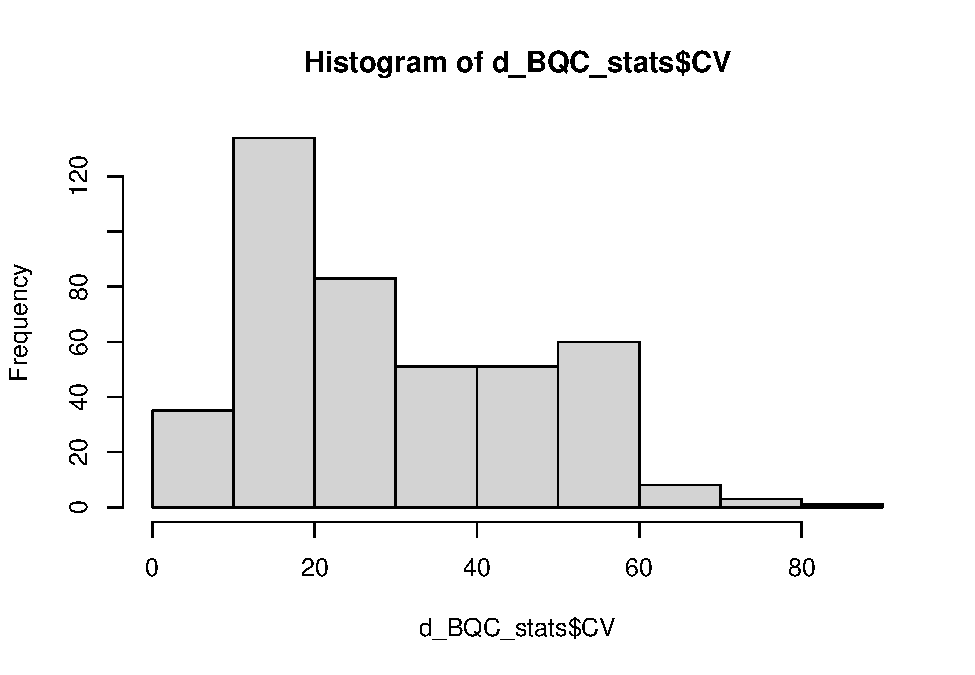
\includegraphics{./datawrangling_files/figure-pdf/calulcate-column-stats-1.pdf}

}

\end{figure}

\begin{Shaded}
\begin{Highlighting}[]
\FunctionTok{hist}\NormalTok{(d\_BQC\_stats}\SpecialCharTok{$}\NormalTok{rCVm)}
\end{Highlighting}
\end{Shaded}

\begin{figure}[H]

{\centering 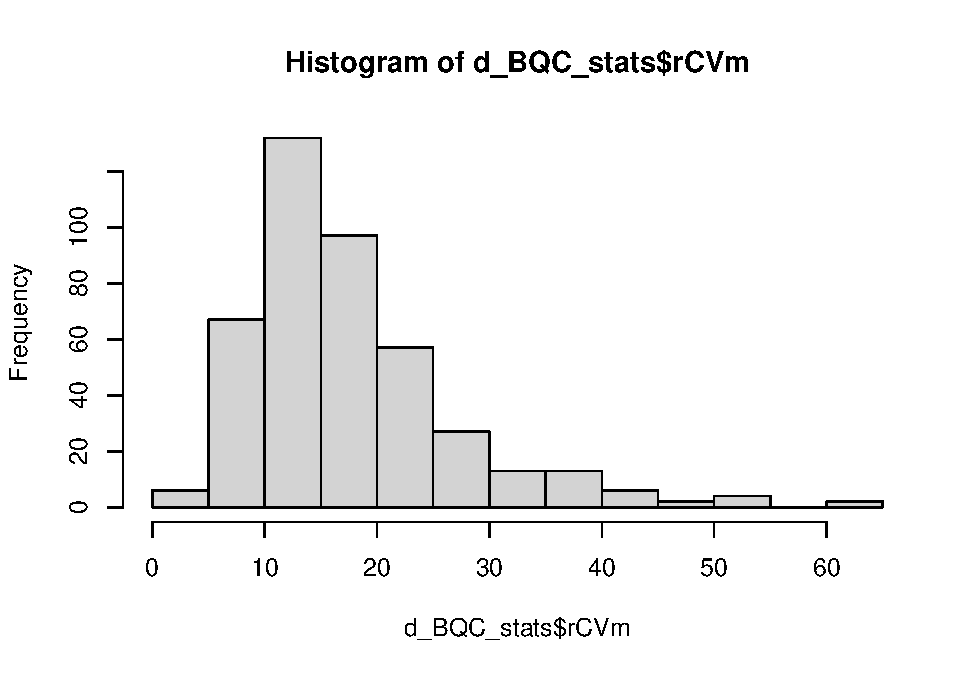
\includegraphics{./datawrangling_files/figure-pdf/calulcate-column-stats-2.pdf}

}

\end{figure}

\begin{Shaded}
\begin{Highlighting}[]

\FunctionTok{ggplot}\NormalTok{(d\_BQC\_stats) }\SpecialCharTok{+}
  \FunctionTok{geom\_histogram}\NormalTok{(}\FunctionTok{aes}\NormalTok{(}\AttributeTok{x=}\NormalTok{CV))}
\CommentTok{\#\textgreater{} \textasciigrave{}stat\_bin()\textasciigrave{} using \textasciigrave{}bins = 30\textasciigrave{}. Pick better value with \textasciigrave{}binwidth\textasciigrave{}.}
\CommentTok{\#\textgreater{} Warning: Removed 2 rows containing non{-}finite values (stat\_bin).}
\end{Highlighting}
\end{Shaded}

\begin{figure}[H]

{\centering 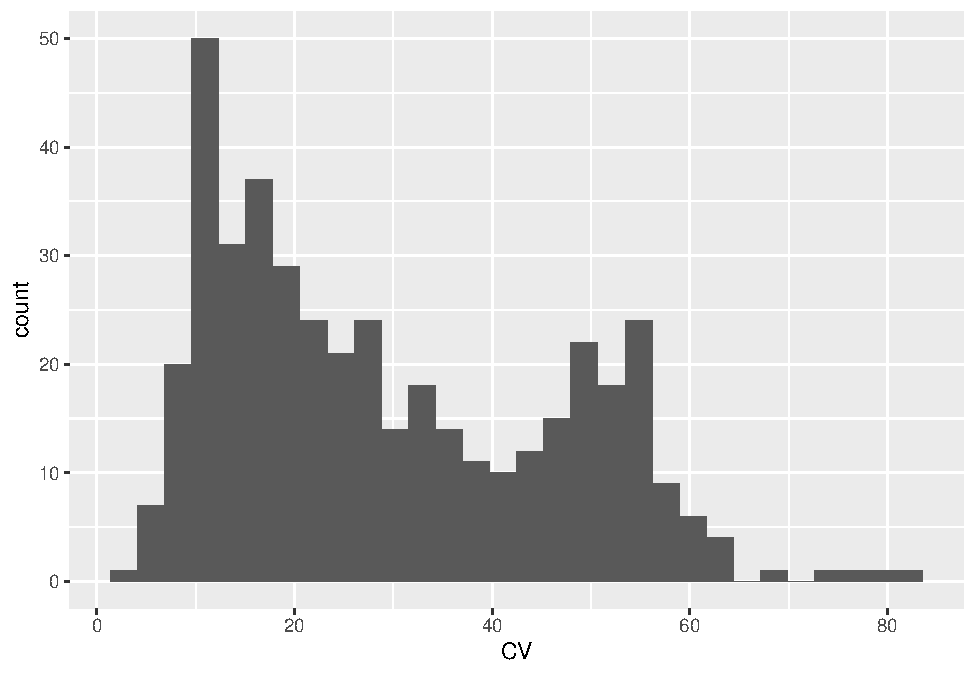
\includegraphics{./datawrangling_files/figure-pdf/calulcate-column-stats-3.pdf}

}

\end{figure}

\begin{Shaded}
\begin{Highlighting}[]

\NormalTok{d\_BQC\_stats\_long }\OtherTok{\textless{}{-}}\NormalTok{ d\_BQC\_stats }\SpecialCharTok{|\textgreater{}}
\NormalTok{  dplyr}\SpecialCharTok{:::}\FunctionTok{select}\NormalTok{(Compound, CV,rCVm,,rCVq, logCV) }\SpecialCharTok{|\textgreater{}} 
  \FunctionTok{pivot\_longer}\NormalTok{(}\AttributeTok{cols =} \SpecialCharTok{{-}}\NormalTok{Compound, }\AttributeTok{names\_to=} \StringTok{"CV\_type"}\NormalTok{ ,}\AttributeTok{values\_to =} \StringTok{"Value"}\NormalTok{)}
\NormalTok{d\_BQC\_stats\_long}
\CommentTok{\#\textgreater{} \# A tibble: 1,712 x 3}
\CommentTok{\#\textgreater{}   Compound CV\_type Value}
\CommentTok{\#\textgreater{}   \textless{}chr\textgreater{}    \textless{}chr\textgreater{}   \textless{}dbl\textgreater{}}
\CommentTok{\#\textgreater{} 1 CE 14:0  CV       18.8}
\CommentTok{\#\textgreater{} 2 CE 14:0  rCVm     12.9}
\CommentTok{\#\textgreater{} 3 CE 14:0  rCVq     13.4}
\CommentTok{\#\textgreater{} 4 CE 14:0  logCV    21.3}
\CommentTok{\#\textgreater{} \# ... with 1,708 more rows}

\FunctionTok{ggplot}\NormalTok{(d\_BQC\_stats\_long) }\SpecialCharTok{+}
  \FunctionTok{geom\_histogram}\NormalTok{(}\FunctionTok{aes}\NormalTok{(}\AttributeTok{x=}\NormalTok{Value, }\AttributeTok{fill =}\NormalTok{ CV\_type)) }\SpecialCharTok{+} \FunctionTok{scale\_x\_continuous}\NormalTok{(}\AttributeTok{limits =} \FunctionTok{c}\NormalTok{(}\DecValTok{0}\NormalTok{,}\DecValTok{150}\NormalTok{)) }\SpecialCharTok{+} \FunctionTok{facet\_wrap}\NormalTok{(}\SpecialCharTok{\textasciitilde{}}\NormalTok{CV\_type)}
\CommentTok{\#\textgreater{} \textasciigrave{}stat\_bin()\textasciigrave{} using \textasciigrave{}bins = 30\textasciigrave{}. Pick better value with \textasciigrave{}binwidth\textasciigrave{}.}
\CommentTok{\#\textgreater{} Warning: Removed 22 rows containing non{-}finite values (stat\_bin).}
\CommentTok{\#\textgreater{} Warning: Removed 8 rows containing missing values (geom\_bar).}
\end{Highlighting}
\end{Shaded}

\begin{figure}[H]

{\centering 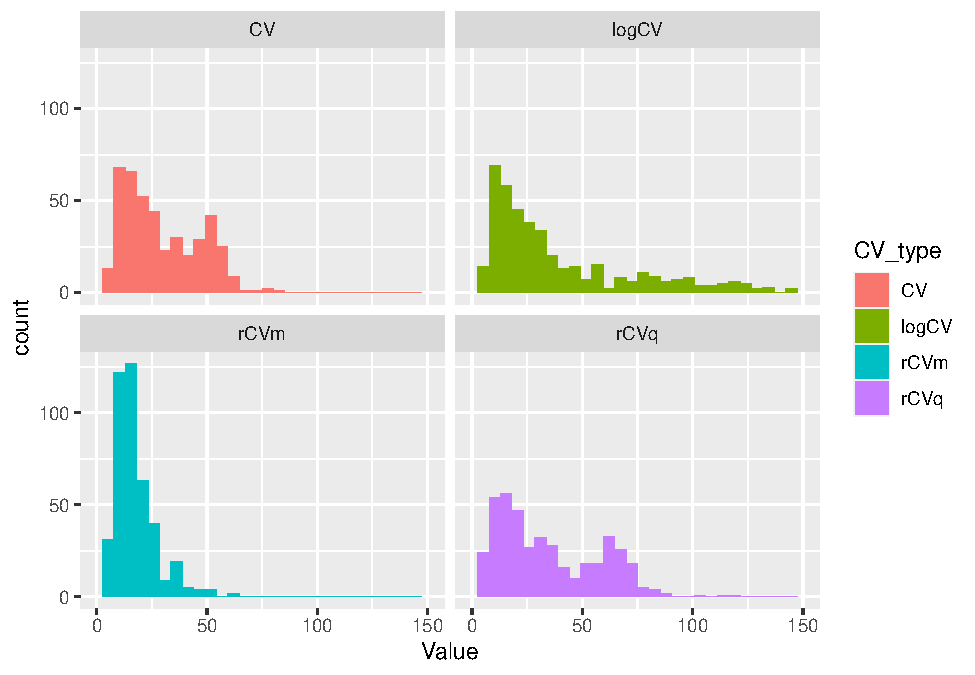
\includegraphics{./datawrangling_files/figure-pdf/calulcate-column-stats-4.pdf}

}

\end{figure}

\begin{Shaded}
\begin{Highlighting}[]


\FunctionTok{plot}\NormalTok{(d\_BQC\_stats}\SpecialCharTok{$}\NormalTok{CV, d\_BQC\_stats}\SpecialCharTok{$}\NormalTok{logCV)}
\end{Highlighting}
\end{Shaded}

\begin{figure}[H]

{\centering 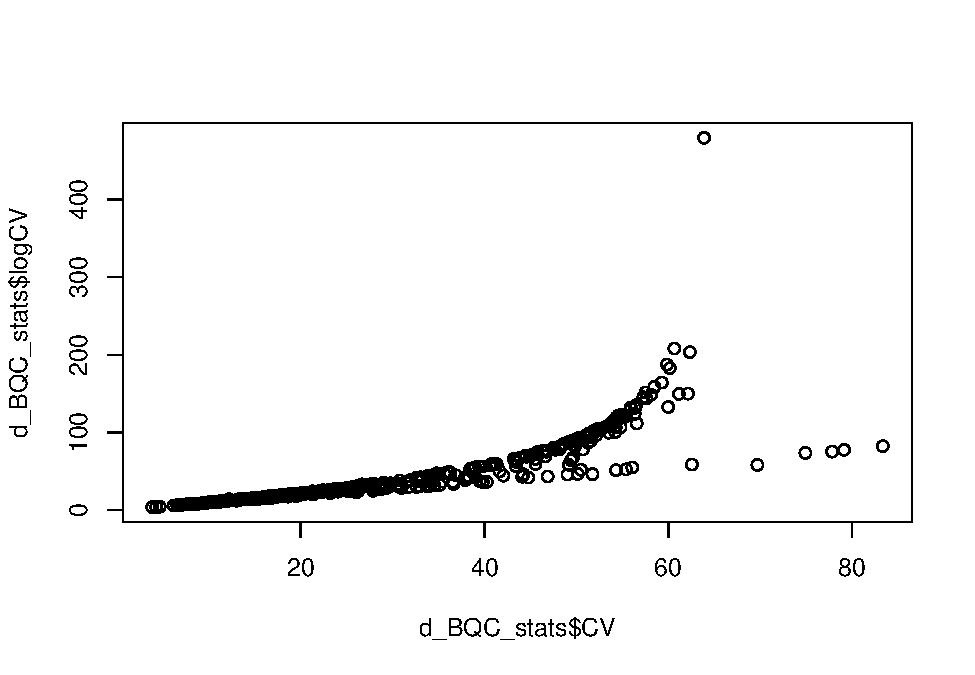
\includegraphics{./datawrangling_files/figure-pdf/calulcate-column-stats-5.pdf}

}

\end{figure}

\begin{Shaded}
\begin{Highlighting}[]
\FunctionTok{plot}\NormalTok{(d\_BQC\_stats}\SpecialCharTok{$}\NormalTok{CV, d\_BQC\_stats}\SpecialCharTok{$}\NormalTok{logCV, }\AttributeTok{xlim =} \FunctionTok{c}\NormalTok{(}\DecValTok{0}\NormalTok{,}\DecValTok{100}\NormalTok{), }\AttributeTok{ylim =} \FunctionTok{c}\NormalTok{(}\DecValTok{0}\NormalTok{,}\DecValTok{100}\NormalTok{))}
\end{Highlighting}
\end{Shaded}

\begin{figure}[H]

{\centering 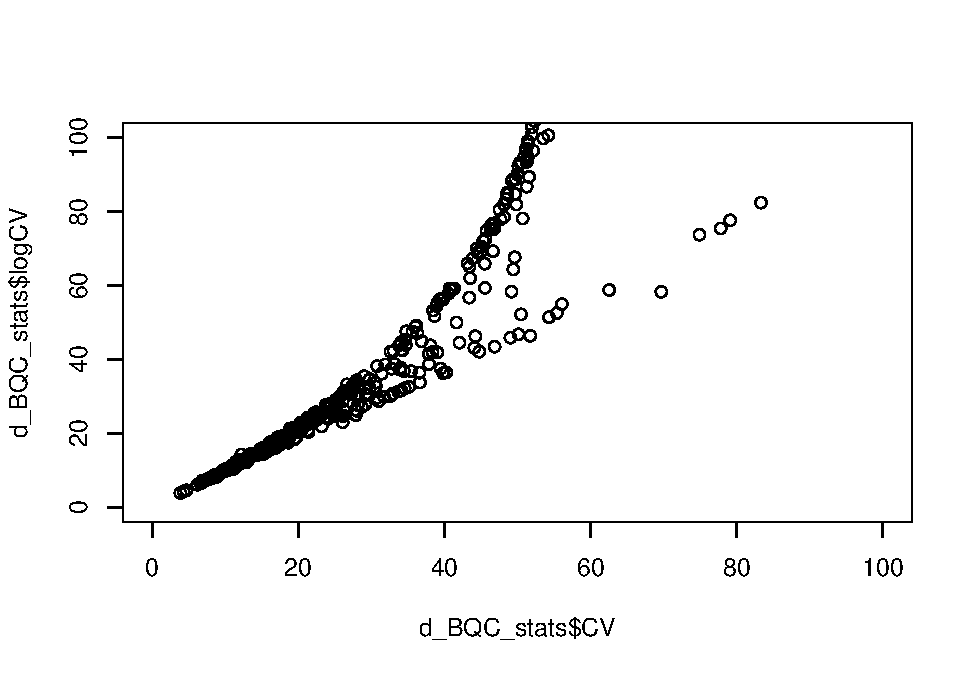
\includegraphics{./datawrangling_files/figure-pdf/calulcate-column-stats-6.pdf}

}

\end{figure}

\begin{Shaded}
\begin{Highlighting}[]
\FunctionTok{plot}\NormalTok{(d\_BQC\_stats}\SpecialCharTok{$}\NormalTok{CV, d\_BQC\_stats}\SpecialCharTok{$}\NormalTok{rCVm)}
\end{Highlighting}
\end{Shaded}

\begin{figure}[H]

{\centering 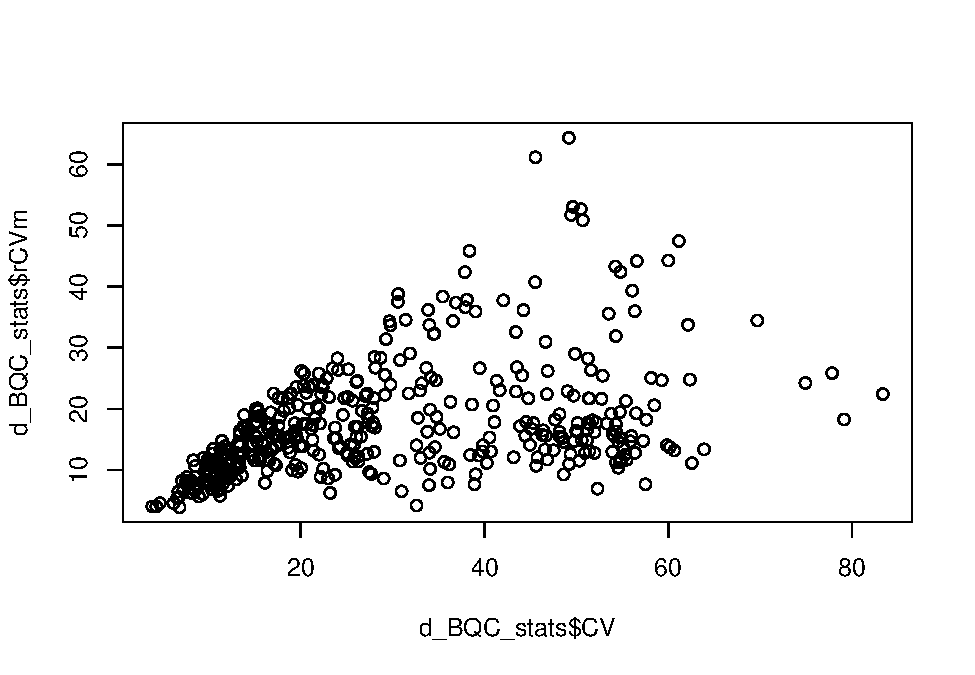
\includegraphics{./datawrangling_files/figure-pdf/calulcate-column-stats-7.pdf}

}

\end{figure}

\begin{Shaded}
\begin{Highlighting}[]
\FunctionTok{plot}\NormalTok{(d\_BQC\_stats}\SpecialCharTok{$}\NormalTok{logCV, d\_BQC\_stats}\SpecialCharTok{$}\NormalTok{rCVm, }\AttributeTok{xlim =} \FunctionTok{c}\NormalTok{(}\DecValTok{0}\NormalTok{,}\DecValTok{200}\NormalTok{))}
\end{Highlighting}
\end{Shaded}

\begin{figure}[H]

{\centering 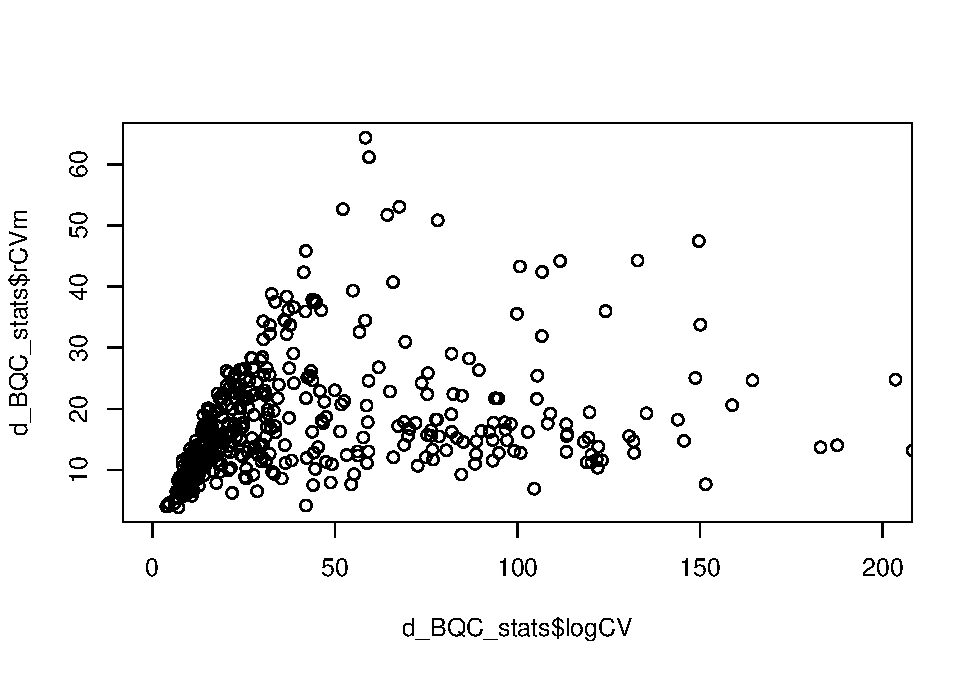
\includegraphics{./datawrangling_files/figure-pdf/calulcate-column-stats-8.pdf}

}

\end{figure}

\begin{Shaded}
\begin{Highlighting}[]
\FunctionTok{plot}\NormalTok{(d\_BQC\_stats}\SpecialCharTok{$}\NormalTok{CV, d\_BQC\_stats}\SpecialCharTok{$}\NormalTok{rCVq)}
\end{Highlighting}
\end{Shaded}

\begin{figure}[H]

{\centering 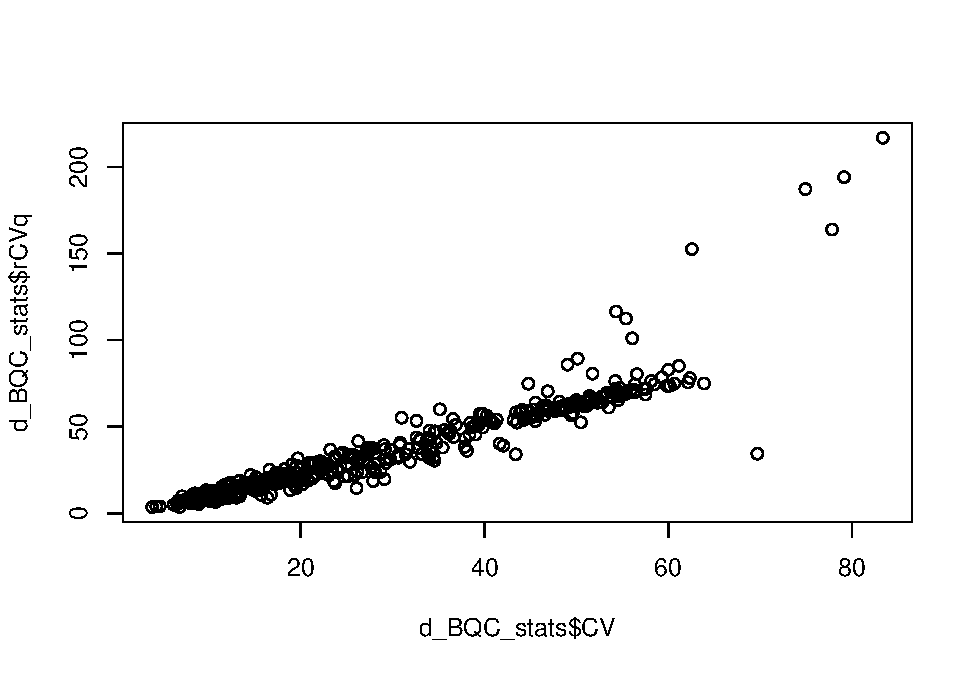
\includegraphics{./datawrangling_files/figure-pdf/calulcate-column-stats-9.pdf}

}

\end{figure}

\hypertarget{summary}{%
\chapter{Summary}\label{summary}}

In summary, this book has no content whatsoever.

\begin{Shaded}
\begin{Highlighting}[]
\DecValTok{1} \SpecialCharTok{+} \DecValTok{1}
\end{Highlighting}
\end{Shaded}

\begin{verbatim}
[1] 2
\end{verbatim}

\hypertarget{references}{%
\chapter*{References}\label{references}}
\addcontentsline{toc}{chapter}{References}

\hypertarget{refs}{}
\begin{CSLReferences}{0}{0}
\end{CSLReferences}



\end{document}
